% =====================================================================
% MARSA -- Master's Thesis Monograph (MISIS, Universidad de los Andes)
% Tomas Acosta Bernal
% =====================================================================
\documentclass[11pt]{report}

\usepackage[utf8]{inputenc}
\usepackage[T1]{fontenc}
\usepackage{lmodern}
\usepackage[margin=1in]{geometry}
\usepackage{placeins}
\usepackage{float}
\usepackage{booktabs}
\usepackage{graphicx}
\usepackage{amsmath,amssymb}
\usepackage{siunitx}
\usepackage{multirow}
\usepackage{array}
\usepackage{xcolor}
\usepackage{tikz}
\usetikzlibrary{arrows.meta,positioning,fit,backgrounds}
\usepackage[colorlinks=true,linkcolor=black,citecolor=black,urlcolor=blue]{hyperref}
\usepackage{xurl}
\usepackage[numbers,sort&compress]{natbib}
\bibliographystyle{unsrtnat}

% Flag for items that are genuinely not finished yet (same convention as
% IEEE/main.tex).
\newcommand{\PENDING}[1]{\textcolor{red}{\textbf{[PENDING: #1]}}}

\title{\textbf{MARSA: A Multi-accent Corpus of Full and Partial Voice
Spoofing Attacks for Spanish Anti-spoofing Research}}

\author{Tom\'as Acosta Bernal}
\date{November 20, 2026}

\begin{document}

% =====================================================================
% Title page
% =====================================================================
\begin{titlepage}
\centering
\vspace*{1cm}
{\large Universidad de los Andes\\
Department of Systems and Computing Engineering\\
FLAG Lab\par}
\vspace{2cm}
{\Large\bfseries Master's Thesis\par}
\vspace{1cm}
{\huge\bfseries MARSA: A Multi-accent Corpus of Full and Partial Voice
Spoofing Attacks for Spanish Anti-spoofing Research\par}
\vspace{2cm}
{\Large Tom\'as Acosta Bernal\par}
\vspace{0.5cm}
{\large November 20, 2026\par}
\vfill
{\large This thesis is submitted in partial fulfillment of the
requirements for the degree of Master in Systems and Computing
Engineering.\par}
\vspace{1cm}
\begin{flushleft}
\textbf{Advisor:}\\
Prof. Rub\'en Francisco Manrique \hfill Universidad de los Andes, Colombia
\end{flushleft}
\end{titlepage}

\begin{abstract}
\noindent
Neural text-to-speech (TTS) and voice-cloning technology increasingly
enable voice-based fraud, impersonation, and disinformation, extending
beyond defeating automatic speaker verification (ASV) systems. The
same technology drives identity theft, fraudulent phone calls that
impersonate a trusted contact, fabricated audio misattributed to public
figures, and cloned voice messages circulated on messaging platforms.
Despite the aforementioned problems, the datasets used to build and
benchmark spoofing countermeasures are predominantly English or
Mandarin, whereas Spanish (the world's second most-spoken native
language, with more than 500 million native speakers
\citep{cervantes2025espanol}) has had no
large-scale, openly available anti-spoofing corpus to capture both
full-utterance synthesis and partial (word-level) manipulation. We
introduced \textbf{MARSA} (Multi-accent Audio Recordings for Spanish
Anti-spoofing), a corpus of 240{,}995 utterances built from 35{,}927
bonafide recordings spanning seven Spanish accents across Spain and
Latin America. MARSA comprises three tiers: (1) 186{,}647 full-spoof
utterances generated by six state-of-the-art open TTS voice-cloning
systems. (2) 18{,}421 partial-spoof utterances, in which one to three
words of an otherwise bonafide recording are replaced by cloned speech
using an energy-aware splicing engine. (3) An acoustic-augmentation
layer covering reverberation, additive noise, and telephony/VoIP
codecs at four multiplicative factors. All data are released in the
ASVspoof2019 Logical Access protocol format, including frame-level
spoof labels for the partial spoof tier, as well as system-level
identifiers that link each spoofed utterance to its generating
algorithm and, for partial spoof samples, to the corresponding
replacement tier and splice variant. These identifiers give MARSA
support for multi-class attack-type attribution and source-tracing
identification in addition to bonafide vs. spoof detection. A zero-shot
evaluation of four existing anti-spoofing detectors against MARSA
confirms that it functions as a discriminating benchmark and exposes a
sharp generalization gap, especially on the partial-spoof tier. Its
suitability for training new detectors is left to future work. In
addition, MARSA supports
the cross-condition benchmarking of Spanish anti-spoofing detectors,
and, more broadly, the study of how language and dialect affect the
generalization of spoofing countermeasures.
\end{abstract}

\chapter*{Acknowledgements}
I am deeply grateful to my advisor, Prof. Rub\'en Francisco Manrique,
for supporting me throughout the development of this thesis, and for
making it possible for me to pursue this master's degree in the first
place.

\begin{center}
\emph{``En nombre de Marsa, madre, hermana y abuela de 14 nietos.''}
\end{center}

MARSA carries this name in honor of my mother and my grandmother, who
share it. This thesis, and the corpus at its center, is dedicated to
both of them.

I am also deeply grateful to my father, for his support throughout
this process and for giving me every reason to want to make him
proud.

\tableofcontents
\listoffigures
\listoftables

% =====================================================================
\chapter{Introduction}
\label{ch:introduction}

\section{Context}

Voice cloning threatens more than biometric authentication.
The same technology enables identity theft and impersonation of private
individuals, fabricated audio misattributed to public figures for
disinformation, fraudulent phone calls that impersonate a trusted contact
to extract money or information
\citep{forbes2019ceofraud,destefano2023testimony,europol2022deepfakes}, and
cloned voice messages circulated on messaging platforms
\citep{infobae2026whatsapp}. These threats are well documented in Latin
America, where police statistics and journalistic reporting describe
rising voice-cloning extortion and family-impersonation scams
\citep{infobae2025colombia,infobae2026whatsapp}. The damage also reaches
listeners who are never deceived. A listening study of 35{,}532 human
judgments across 138 synthesis systems found that, as synthetic speech
improved, human accuracy at identifying genuine recordings fell sharply
(72.7\% to 64.1\%), whereas accuracy at catching fakes stayed comparatively
stable (72.9\% to 71.2\%) \citep{muller2026erodingtrust}. This erosion of
trust in authentic audio compounds the direct fraud risk.

ASV bypass is nonetheless the best-studied instance of this
threat, because it is the only setting with standardized, large-scale
benchmarks. A related line of work, Spoofing-Aware Speaker Verification
(SASV), jointly optimizes speaker verification and spoof detection rather
than treating them as independent subsystems
\citep{sasvevalplan2022,sasv2022,Wu2026wildspoof}. All these settings share
the same synthesis technology and the same countermeasures; a corpus
built for ASV-focused detection therefore transfers directly to detecting synthetic
or manipulated speech in non-biometric contexts.

The ASVspoof challenge series established the standard datasets and
evaluation protocols for voice anti-spoofing research
\citep{asvspoof2019,asvspoof2021,asvspoof5}. A large body of work has
since developed neural countermeasures such as RawNet2, wav2vec\,2.0
front-ends, and graph-attention detectors \citep{rawnet2,tak2022ssl,aasist}.
More recent work has moved toward larger self-supervised backbones
\citep{vasquez2026wildspoof} and dedicated benchmarking infrastructure for
comparing them, including compact-backbone studies such as RAPTOR
\citep{raptor2026} and the Speech DF Arena leaderboard
\citep{dowerah2025speechdfarena}.

\section{Problem Statement}

Almost all of this progress has been measured in English. The datasets
that anchor anti-spoofing research are, with few exceptions, English (the
ASVspoof Logical Access sets derive from English source speech) or
Mandarin (the Half-Truth partial-fake corpus \citep{yi2021had}). Recent
large multilingual corpora such as MLAAD \citep{mlaad} and SpeechFake
\citep{speechfake} do include Spanish, but only as one of dozens of
languages, with a single accent per language and without a partial-spoof
or dialect-stratified design. The one dedicated Spanish resource,
HISPASpoof \citep{hispaspoof}, provides real and fully synthesized speech
in six accents, but is limited to full-utterance synthesis, with no
partial-spoof tier, no boundary-shortcut control, and no
acoustic-augmentation layer. The initial HABLA dataset \citep{habla} was
an early step toward Latin American Spanish anti-spoofing, but is limited
in speaker count, accent coverage, and attack diversity, and does not
address partial spoofing.

No existing resource combines large-scale, cross-continental Spanish
coverage with full spoofing, partial spoofing, and a channel-augmentation
layer. Most related studies also cast the problem as binary detection
(bonafide vs.\ spoof) without recording which generation algorithm
produced each spoofed utterance. Attack-type attribution matters for
forensic response and for tracking which synthesis methods attackers
actively use, yet beyond the full-utterance setting it has little data
to work with. Datasets built around a single
generation family, most notably ASVspoof2019 itself
\citep{asvspoof2019}, already assign a system-level label to each
full-utterance attack, but this granularity has not extended to
partial, word-level splices, where the generating system, replacement
tier, and splice technique of each edit are rarely all recorded
together. Section~\ref{sec:sota} (State of the Art) compares MARSA
against the closest existing corpora in detail.

\section{Justification}

Language affects spoofing detection. Cross-dialectal
acoustic variation within Spanish degrades state-of-the-art speech models
non-uniformly. Even though an accent classifier trained on raw acoustics
struggles to separate several of these varieties given their close
phonological similarity \citep{zuluaga2023commonaccent}, automatic speech
recognition (ASR) word error rates (WER) still differ by several absolute
points across Argentine, Chilean, Colombian, Mexican, Peninsular, and
Peruvian Spanish \citep{kantharuban2023dialectgap,nacimiento2024biases}.
We therefore cannot assume that a spoofing
detector, which must decide whether a signal is genuine and, for partial
spoofing, which segments are genuine, transfers across these varieties.
Dialect-robust Spanish anti-spoofing requires a corpus that accounts for
this variation.

Partial spoofing replaces a short span of an otherwise
genuine utterance with synthetic speech. Because most of the signal
remains authentic, it is a distinct and harder threat than full synthesis
\citep{zhang2023partialspoof}. Dedicated challenges such as the
partially-fake track of ADD 2022 \citep{add2022} have targeted it, and it
is also the threat for which Spanish resources are scarcest. The only
multilingual partial-spoof benchmark that includes Spanish, HQ-MPSD
\citep{li2025hqmpsd}, generates its partial-spoof utterances with a
single TTS system and a single splice method, drawn from 155,145
utterances pooled across eight languages with no published
per-language breakdown; consequently, the Spanish-specific scale cannot be stated
precisely. It does draw multiple speakers per language to vary accent,
and combines reverberation and noise conditions, but offers no
partial-spoof boundary-shortcut control. Prior forensic work shows that partial-spoof detectors can
exploit a shortcut. Because only the boundaries flanking the spliced
segment are anomalous, a detector can learn to find the discontinuous
boundary instead of the synthesis artifact and still achieve low error
without ever learning the actual spoofing cue
\citep{negroni2024splicing,huang2024detectable}. A corpus intended for
robust detection must therefore control for this shortcut.

\section{Objectives}

\subsection{General Objective}

To construct, validate, and publicly release a large-scale, multi-accent
Spanish corpus of full and partial voice spoofing attacks, suitable for
training and benchmarking anti-spoofing countermeasures under realistic
acoustic channel conditions.

\subsection{Specific Objectives}

\begin{enumerate}
  \item To build a bonafide source corpus covering seven Spanish accents
  across two continents, combining the existing HABLA corpus with a
  Mozilla Common Voice extension to fill under-represented accent groups.
  \item To generate a full-spoof tier using six independent, open-source
  neural TTS voice-cloning systems, screened for intelligibility,
  perceptual quality, and speaker fidelity.
  \item To design and implement an energy-aware splicing engine that
  produces a partial-spoof tier (one-to-three word replacements) with a
  boundary-jitter variant explicitly designed to suppress the
  splice-boundary detector shortcut documented in prior forensic work.
  \item To build an acoustic-augmentation layer covering reverberation,
  additive noise, and telephony/VoIP codec degradation at multiple
  multiplicative factors, so that channel robustness can be studied
  without regenerating attacks.
  \item To release every tier in a standardized, attack-attributed
  protocol format compatible with existing anti-spoofing training and
  evaluation code, and to validate the corpus through intrinsic quality
  metrics and zero-shot baseline anti-spoofing detection.
\end{enumerate}

\subsection*{Publication Derived from This Thesis}
\begin{itemize}
  \item Acosta Bernal, T., V\'asquez Correa, J.C., Calder\'on Acosta,
  M.D., Manrique, R.F. \emph{MARSA: A Multi-accent Corpus of Full and
  Partial Voice Spoofing Attacks for Spanish Anti-spoofing Research.}
  Submitted to \emph{Scientific Data} (Nature Portfolio) on November 6,
  2026; under review.
\end{itemize}

% =====================================================================
\chapter{Conceptual Framework and State of the Art}
\label{ch:background}

\section{Conceptual Framework}

This section introduces the vocabulary and basic technical concepts used
throughout the rest of the thesis. Readers already familiar with speech
synthesis and anti-spoofing terminology can skip to
Section~\ref{sec:sota}.

\subsection{Speech Synthesis and Voice Conversion}

Two distinct technologies can be used to generate a spoofed speech sample.
\textbf{Text-to-speech (TTS)} synthesis produces spoken output directly
from written text, without requiring any genuine recording of the target
speaker at generation time beyond whatever reference audio the model was
conditioned on; the attacker steals the target's identity directly from
text. \textbf{Voice conversion (VC)} instead requires two real referents:
a source speaker, whose recorded performance supplies the linguistic
content and manner of speaking, and a target speaker, whose
non-linguistic characteristics (timbre) the system imposes on that
performance so that the result sounds like the target saying what the
source said. Both attack types can be mounted against an ASV system's
logical access point. MARSA's full-spoof tier instantiates only the TTS
attack type: all six generating systems synthesize speech directly from
text conditioned on a target reference, with no second human source
speaker involved. OpenVoice v2 applies a tone-conversion module as a
postprocessing step, but its input is itself TTS-generated audio rather
than a genuine source recording, which means this is not two-referent voice
conversion as defined above. Genuine recording-to-recording voice
conversion is outside MARSA's current scope (Chapter~\ref{ch:methods}).

\textbf{Partial spoofing} is a third manipulation. Instead
of synthesizing an entire utterance, it replaces a short span (here, one
to three words) of a genuine recording with synthetic speech
and leaves the rest of the signal authentic \citep{zhang2023partialspoof}.
MARSA's partial-spoof tier targets this manipulation.

\subsection{Anti-spoofing Countermeasures}

An anti-spoofing countermeasure (CM) is a classifier that decides whether
an input utterance is \emph{bonafide} (genuine) or \emph{spoofed}. Most CM
architectures are composed of a \textbf{front-end}, which extracts an
acoustic feature representation from the raw waveform, and a
\textbf{back-end}, which maps that feature sequence to a bonafide/spoof
decision. Common front-ends include Mel-Frequency Cepstral Coefficients
(MFCC), Linear-Frequency Cepstral Coefficients (LFCC), Constant-Q
Cepstral Coefficients (CQCC), and raw spectrograms; common back-ends
include Light Convolutional Neural Networks (LCNN), recurrent
architectures, and, increasingly, self-supervised representations fed
into a lightweight classification head \citep{rawnet2,tak2022ssl,aasist}.

\subsection{Evaluation Metric: Equal Error Rate}

Countermeasures are conventionally evaluated with the \textbf{Equal Error
Rate (EER)}: the operating point at which the system's False Rejection
Rate (the fraction of genuine utterances incorrectly flagged as spoofed)
equals its False Acceptance Rate (the fraction of spoofed utterances
incorrectly accepted as genuine). A lower EER indicates better
discrimination between bonafide and spoofed utterances; an EER of 0\%
would mean perfect separation at some threshold. MARSA's Technical
Validation (Chapter~\ref{ch:evaluation}) reports zero-shot EER for
several existing CM architectures evaluated directly against the corpus,
without retraining on it.

\subsection{Corpus Release Convention}

MARSA follows the ASVspoof2019 Logical Access (LA) release convention: a
flat directory of audio files per split (train/dev/eval), accompanied by
a protocol file that records, for every utterance, its speaker, a unique
audio identifier, the generating system (or a placeholder for bonafide
audio), and the bonafide/spoof label. This convention is widely used by
existing anti-spoofing training and evaluation code, which is why MARSA
adopts it rather than a corpus-specific format
(Chapter~\ref{ch:data-records}).

\section{State of the Art}
\label{sec:sota}

Almost none of the anti-spoofing literature surveyed in the Context
section of Chapter~\ref{ch:introduction} is in Spanish. The datasets that
anchor anti-spoofing research are, with few exceptions, English or
Mandarin (the Half-Truth partial-fake corpus \citep{yi2021had}).
Table~\ref{tab:corpuscompare}
compares MARSA against the closest existing Spanish, accent-stratified
corpora; Table~\ref{tab:multilingualcompare} separately compares it
against large multilingual synthetic-speech collections that include
Spanish only as one of dozens of languages, which are measured on
different axes (language coverage, total synthetic-audio hours) and are
not directly comparable to the accent-stratified corpora in the first
table.

\begin{table}[H]
\centering
\caption{MARSA compared with the closest existing Spanish, accent-stratified
anti-spoofing corpora. Systems is the number of distinct generating
systems (TTS/VC) reported by the source. HABLA's bonafide and
full-spoof counts are reported as approximate in the source
publication. Aug.: dedicated acoustic-augmentation layer
(reverberation, noise, codec).}
\label{tab:corpuscompare}
\small
\begin{tabular}{lcccccc}
\toprule
\textbf{Corpus} & \textbf{Accents} & \textbf{Bonafide} & \textbf{Systems} & \textbf{Full-spoof} & \textbf{Partial-spoof} & \textbf{Aug.} \\
\midrule
HABLA \citep{habla}      & 5 & 22{,}000 & 4 & 58{,}000 & No & No \\
HISPASpoof \citep{hispaspoof} & 6 & 6{,}241  & 6 & 37{,}446 & No & No \\
\textbf{MARSA (this work)} & \textbf{7} & \textbf{35{,}927} & \textbf{6} & \textbf{186{,}647} & \textbf{18{,}421} & \textbf{Yes} \\
\bottomrule
\end{tabular}
\end{table}

\begin{table}[H]
\centering
\caption{MARSA compared with large multilingual synthetic-speech
collections. These are not accent-stratified Spanish anti-spoofing
corpora (Table~\ref{tab:corpuscompare}); they are measured here on the
axes their own publications report: language coverage, number of
generating systems, and total synthetic-audio scale across every
covered language, not Spanish alone. Spanish-specific gives whether
the corpus stratifies its Spanish-language content by accent. MARSA's
248.8~h is the sum of its full-spoof (218.6~h) and partial-spoof
(30.2~h) tiers; it excludes bonafide audio and the augmentation tiers,
which are multiplicative copies of this base and would make the figure
dependent on which augmentation factor is chosen.}
\label{tab:multilingualcompare}
\small
\begin{tabular}{lcccc}
\toprule
\textbf{Corpus} & \textbf{Languages} & \textbf{Systems} & \textbf{Synthetic audio} & \textbf{Spanish-specific} \\
\midrule
MLAAD \citep{mlaad}           & 54 & 205 & 1{,}153.6 h        & No \\
SpeechFake \citep{speechfake} & 46 & 40  & $>$3{,}000 h       & No \\
\textbf{MARSA (this work)}    & \textbf{1} & \textbf{6} & \textbf{248.8 h} & \textbf{Yes (7 accents)} \\
\bottomrule
\end{tabular}
\end{table}

Table~\ref{tab:overview} summarizes the main aspects of the introduced
MARSA corpus. The following chapters detail how each tier was produced
(Chapter~\ref{ch:methods}), how the release is organized on disk
(Chapter~\ref{ch:data-records}), the quality and baseline-detection
evidence that the data are fit for purpose
(Chapter~\ref{ch:evaluation}), and practical guidance for reuse
(Chapter~\ref{ch:discussion}).

\begin{table}[H]
\centering
\caption{MARSA corpus overview. Augmentation is released as four
separate tiers, each a full copy of the base corpus at the stated
multiplication factor (for example, the $\times$5 tier holds five times
the base utterance count and five times the base hours); a user selects
one factor rather than combining them. Duration refers to the average duration (in seconds) of each utterance.}
\label{tab:overview}
\small
\begin{tabular}{lrrlp{5.5cm}}
\toprule
\textbf{Tier} & \textbf{Utt.} & \textbf{Hours} & \textbf{Duration ($\sigma$)}  & \textbf{Description} \\
\midrule
Bonafide            & 35{,}927  & 53.8  & 5.39 (1.62)  & Source corpus, 7 accents, 1{,}567 speakers \\
Full spoof          & 186{,}647 & 218.6 & 4.22 (1.19)  & 6 TTS voice-cloning systems \\
Partial spoof       & 18{,}421  & 30.2  & 5.90 (1.61)  & 1--3 word replacements (15{,}641 clean) \\
\midrule
\textbf{Base total} & \textbf{240{,}995} & \textbf{302.6} & 4.52 &  Pre-augmentation \\
\midrule
Augmented tiers & \multicolumn{3}{l}{$\times$2 / $\times$3 / $\times$5 / $\times$10 the base row above} & Released separately per factor \\
\bottomrule
\end{tabular}
\end{table}

% =====================================================================
\chapter{Corpus Construction Methodology}
\label{ch:methods}

\section{Bonafide Source Corpus}
\label{sec:bonafide}

The genuine-speech foundation of MARSA combines the original HABLA Latin
American Spanish anti-spoofing dataset \citep{habla} with additional
speakers drawn from Mozilla Common Voice \citep{commonvoice} added to
fill the accent groups HABLA under-represents. Candidate Common Voice
speakers were embedded with the same ECAPA-TDNN model used throughout
MARSA for speaker-similarity screening \citep{ecapa}
(Chapter~\ref{ch:evaluation}), and any candidate whose cosine similarity
to an existing HABLA speaker reached 0.75 or higher was excluded, to
avoid admitting near-duplicate voices across the two sources. This
threshold was set by listening validation during pipeline development.
Pairs scoring at or above 0.75 were, by ear, difficult to tell apart as
different speakers. Peninsular
and Mexican Spanish speakers are drawn entirely from this Common Voice
extension. Colombian and Chilean speakers are a blend of both sources.
Argentine and Peruvian speakers are unchanged from the original HABLA
release.

The bonafide data comprise 35{,}927 utterances from 1{,}567 speakers, each
labeled with one of seven accent codes. The accent distribution is given
in Table~\ref{tab:accents}. Two properties are important for downstream
use. First, the corpus is \emph{cross-continental}: Peninsular Spanish is
the single largest accent group (33.7\% of speakers), alongside six Latin
American varieties. Second, the distribution is markedly imbalanced. The
three largest accents (Peninsular, Mexican, Colombian) account for 82.4\%
of the speakers, while the three smallest (Argentine, Peruvian,
Venezuelan) together account for 6.6\% of speakers. Utterance counts do
not track this speaker imbalance. Six of the seven accents land within a
narrow band of 5{,}446--5{,}460 utterances regardless of how many speakers
were available, because each accent subset was built toward a roughly
fixed utterance total rather than a fixed speaker count. Only Venezuelan
is below the total number of utterances (3{,}221). The Common Voice
extension could not close that gap. Its Spanish locale contains very few
self-tagged Venezuelan-accent speakers, and only one passed the
speaker-similarity filter. The group's size (23 speakers) is therefore
almost entirely inherited from the original HABLA release (22 of 23).
This imbalance is a property of the source data and is preserved in
MARSA, allowing users to apply their own balancing strategy.

\begin{table}[H]
\centering
\caption{Accent composition of the bonafide source corpus. Speaker share
is not a valid proxy for utterance share, since utterances per speaker
are not constant across accents.}
\label{tab:accents}
\small
\begin{tabular}{lrrr}
\toprule
\textbf{Accent} & \textbf{Speakers} & \textbf{Utterances} & \textbf{Speaker Share} \\
\midrule
es (Peninsular, Spain) & 528 & 5{,}450 & 33.7\% \\
mx (Mexican)           & 406 & 5{,}450 & 25.9\% \\
co (Colombian)         & 357 & 5{,}450 & 22.8\% \\
cl (Chilean)           & 173 & 5{,}450 & 11.0\% \\
ar (Argentine)         & 42  & 5{,}460 & 2.7\% \\
pe (Peruvian)          & 38  & 5{,}446 & 2.4\% \\
ve (Venezuelan)        & 23  & 3{,}221 & 1.5\% \\
\midrule
\textbf{Total}         & \textbf{1{,}567} & \textbf{35{,}927} & \textbf{100\%} \\
\bottomrule
\end{tabular}
\end{table}

All audio is processed at \SI{16}{\kilo\hertz}, mono, 16-bit. Every
bonafide utterance is transcribed with the Parakeet TDT multilingual
transducer \citep{tdt,parakeet}, which natively emits word-level start
and end timestamps (for partial spoof generation) through its
token-and-duration architecture. Transcription accuracy is validated in
Chapter~\ref{ch:evaluation}. Utterances shorter than four words are
excluded from the partial-spoof tier, because four words is the minimum
sentence length at which even the smallest replacement tier can operate
while keeping the spoofed fraction of the utterance, by word count, at
most one quarter.

The 1{,}567 bonafide speakers are partitioned into speaker-disjoint
train, development, and evaluation splits (1{,}257~/~155~/~155 speakers),
matching the ASVspoof2019 Logical Access train/dev/eval convention the
release format follows (Chapter~\ref{ch:data-records}). The
de-duplication above only compares a Common Voice candidate against
existing HABLA speakers at admission time. It does not check
already-admitted speakers against each other, and two speakers who each
individually cleared that gate could therefore still be near-duplicates
of one another. To close this gap, the same 0.75 ECAPA-TDNN similarity
threshold was applied a second time, exhaustively, across every pair of
the 1{,}567 already-admitted bonafide speakers, to catch any such pair
that had landed on opposite sides of the train/dev/eval split. Six pairs
exceeded the threshold: two HABLA pairs, each linking a train speaker to
one dev or eval speaker, at 0.87 and 0.90 cosine similarity, consistent
with the same voice recorded under two session identifiers; and four
Common Voice pairs at 0.77--0.78 cosine similarity, linking two eval
speakers to three already-admitted train speakers. The four speakers on
the dev or eval side of these six pairs, two from HABLA and two from
Common Voice, were moved into train to remove the leak; the three
train-side Common Voice speakers required no change. Re-auditing the
rebuilt partition confirms the
fix. The maximum cross-split similarity anywhere in the corpus falls to
0.74, below the 0.75 threshold itself. Every synthetic tier inherits this
same partition, since each generated utterance is keyed to the bonafide
speaker it was cloned from. No speaker appears in more than one split
anywhere in the corpus.

\section{Full-spoof Generation Pipeline}
\label{sec:fullspoof}

Each bonafide utterance is the cloning target for six independent,
open-source neural TTS voice-cloning systems, selected against four
criteria:
\begin{enumerate}
  \item \textbf{Open availability} for reproducibility.
  \item \textbf{Demonstrated Spanish synthesis capability}.
  \item \textbf{Architectural diversity}, ensuring the corpus does not
  encode the artifacts of a single synthesis family.
  \item \textbf{Release within the 2024--2026 window}, representing
  current practice.
\end{enumerate}
The six systems include Fish-Speech \citep{fishspeech} (identified as
\texttt{fishgram} in MARSA's protocol files), Qwen3-TTS
\citep{qwen3tts}, OpenVoice v2 \citep{openvoice}, Chatterbox
\citep{chatterbox}, OuteTTS \citep{outetts}, and OmniVoice
\citep{omnivoice}. They comprise autoregressive language models,
diffusion language models, and tone-conversion architectures. CosyVoice
\citep{cosyvoice} was evaluated and excluded because it produced
non-Spanish output for Spanish input text. Table~\ref{tab:systems}
summarizes the six architectures, and the following notes give the
configuration that governs each system's artifacts.

\begin{table}[H]
\centering
\caption{Full-spoof systems: synthesis architecture, acoustic backend,
and configuration artifacts. \textbf{RTF}: Real-Time Factor observed on the generation hardware (lower is faster). \textbf{LM}: Language Model}
\label{tab:systems}
\small
\begin{tabular}{p{2.1cm}p{3.5cm}p{7cm}}
\toprule
\textbf{System} & \textbf{Synthesis architecture} & \textbf{Backend and configuration} \\
\midrule
Fish-Speech & Dual autoregressive LM ($\approx$4\,B params) & Firefly-GAN decoder; served over an HTTP API; \SI{15}{\second} concatenated reference; $\approx$20\,k\,h Spanish training \\
Qwen3-TTS & Autoregressive LM & Speaker-embedding (x-vector) conditioning only; full stochastic sampling (temperature, top-$k$, top-$p$, repetition penalty) \\
OpenVoice v2 & Base TTS plus tone conversion & MeloTTS base voice + ToneColorConverter ($\tau=0.3$); fastest (RTF 0.07--0.10); base voice bleeds through, lowering similarity \\
Chatterbox & Autoregressive with classifier-free guidance & EnCodec acoustic tokens + Vocos vocoder; slowest (RTF 31--45) \\
OuteTTS & Autoregressive LM (Qwen3, 0.6\,B) & WavTokenizer discrete audio codes; patched repetition penalty over the last 64 tokens \\
OmniVoice & Diffusion language model & Native \SI{24}{\kilo\hertz} decoder resampled to \SI{16}{\kilo\hertz}; reference text precomputed with Parakeet; $\approx$27.5\,k\,h Spanish training \\
\bottomrule
\end{tabular}
\end{table}

The six systems were chosen to cover distinct generation families,
ensuring the corpus does not encode the fingerprint of a single
synthesis paradigm. Fish-Speech and Qwen3-TTS are autoregressive language
models that predict acoustic tokens, decoded by a GAN vocoder and an
x-vector-conditioned decoder respectively. Fish-Speech runs as a separate
inference server, and Qwen3-TTS is driven in speaker-embedding-only mode
because its concatenated reference clip does not match a paired
reference transcript. Chatterbox is also autoregressive but adds
classifier-free guidance and reconstructs waveforms from EnCodec tokens
through a Vocos vocoder, at the cost of being the slowest system by more
than an order of magnitude. OuteTTS couples a small Qwen3 backbone to
WavTokenizer discrete codes and requires a patched repetition penalty to
avoid token loops. OpenVoice takes a different route entirely,
synthesizing with a fixed MeloTTS base voice and then transferring timbre
with a tone-color converter, which is fast but allows the base voice to
bleed through. OmniVoice is a diffusion LM with the largest Spanish
training footprint of the six; it generates at \SI{24}{\kilo\hertz} and
is conditioned on a reference transcript that was precomputed with
Parakeet to stay within a single ASR stack.

Every system is driven through a common pipeline. First, a per-speaker
reference clip is assembled by concatenating bonafide recordings from
the target speaker up to a required duration (\SI{15}{\second} for most
systems, and \SI{10}{\second} for OmniVoice, whose documentation advises
against longer references). The concatenation stops at the last
recording that fits without overflowing rather than cutting a file
mid-word, and always ends on a short trailing silence, giving the
reference a clean terminal boundary. Second, the target text is
synthesized in the cloned voice. The text is sampled directly from the
original Common Voice sentence pool (Section~\ref{sec:bonafide}),
independent from the specific bonafide utterance being cloned. Third,
the output audio is resampled to \SI{16}{\kilo\hertz} and validated. A
sample first passes three structural checks: the audio file must exist,
its duration must fall within the accepted range, and it must not be
near-silent; a sample failing any of these is discarded as a
generation failure and excluded from the attack counts. The audio is then transcribed with
Parakeet TDT. The autoregressive models occasionally hallucinate at the
beginning of the intended text; this is detected by aligning the
generated audio against the target transcript, trimming the leading
region up to the first word that matches to keep the artifact out of
the corpus, and re-transcribing the trimmed audio. Word error rate
(WER) and character error rate (CER) are then computed against the
target text; samples exceeding WER $>0.15$ or CER $>0.10$ are
regenerated, for up to five rounds, before being abandoned. These
ceilings were set by listening validation during pipeline development
rather than derived from an external benchmark. At MARSA's average
target-text length (10.4 words, Table~\ref{tab:fullspoofdesc}), a WER
of 0.15 corresponds to roughly one to two incorrect words per sentence;
informal listening checks confirmed that errors at this rate did not
disrupt intelligibility. Character-level errors are harder to judge
reliably by ear in isolation; the CER ceiling was therefore set tighter (0.10)
as an additional numeric safeguard rather than calibrated the same way.
In practice both gates were generous. The realized average WER ranges
from 1.06\% to 2.36\% and CER from 0.30\% to 0.85\% across the six
systems (Table~\ref{tab:fullspoof}), well under both ceilings.
Perceptual quality (NISQA MOS) and speaker similarity (ECAPA-TDNN
cosine similarity to the reference) are computed for every accepted
sample and reported in Chapter~\ref{ch:evaluation}, but are not used as
rejection criteria. Each system targets a 1:1 generation ratio, attempting as many attacks
per speaker as that speaker has bonafide recordings; the realized ratio
after quality filtering varies by system's pass rate
(Table~\ref{tab:fullspoofdesc}).
Table~\ref{tab:fullspoofdesc} (Chapter~\ref{ch:data-records}) describes
the resulting content by system (utterance count, duration, target-text
length).

\paragraph{OmniVoice reference handling.} During validation, OmniVoice
occasionally emitted a 200--\SI{600}{\milli\second} fragment of the
reference speaker's voice before the prompt content. This artifact was
traced to how the reference clip was built. When the concatenated
reference happened to end mid-word, OmniVoice's diffusion conditioning
aimed to complete that truncated word at the very start of generation,
adding a fragment of the reference speaker into the output. Only
OmniVoice showed this behavior in practice, consistent with the other
five systems tokenizing or quantizing the reference rather than
extrapolating from its raw trailing edge; the same end-cut condition
exists in all six pipelines, but was not directly tested on the other
five. Building every reference clip to end on a whole file plus
trailing silence removed the cause of the artifact directly.

As a backstop, the quality screen also checks for this
artifact explicitly. The word-alignment trim used for the autoregressive
systems does not work here, because the bleed is sub-syllabic and
transcription never captures it. Instead, the screen measures the RMS
energy of the interval immediately before the first transcribed word and
rejects and regenerates the utterance whenever that interval exceeds a
silence threshold. We avoided trimming because it risks cutting into a
natural vowel onset.

\paragraph{Watermark handling.} By default, two of the
six TTS systems embed a neural steganographic watermark in their output:
Chatterbox embeds a Perth watermark, and OpenVoice embeds a WavMark
payload in the waveform. These watermarks are imperceptible but survive
resampling and re-encoding. A watermark present in some systems' output
and absent from the rest would create a trivial class-label bias, and
anti-spoofing models would learn to detect the watermark instead of the
synthesis artifact \citep{zhang2026impact}. We therefore disabled both watermarkers at generation
time. No released MARSA sample carries a synthesis-system watermark;
consequently, watermarks carry no class information and detection must rely on
synthesis cues.

\paragraph{System-specific pre- and post-processing.} Some
systems require additional handling that shapes their artifacts.
Fish-Speech normalizes the input text before synthesis. OpenVoice
extracts its tone-color speaker embedding from the reference with a
voice-activity detector and falls back to detector-free extraction when
a reference is too short after silence removal. Chatterbox trims
trailing generation noise from each clip using a voice-activity margin.
OuteTTS builds a per-speaker profile (tempo, energy, pitch, and spectral
centroid) from the reference audio and caches it across that speaker's
utterances. We record these steps for reproducibility; none alters the
linguistic content of the generated speech.

\section{Partial-spoof Generation Pipeline}
\label{sec:partialspoof}

The partial-spoof tier replaces one, two, or three words
of a bonafide utterance with cloned counterparts and leaves the remainder
genuine. The number of replaced words defines three difficulty tiers: W1
(one), W2 (two), and W3 (three). Sentence length determines tier
eligibility (at least 4, 8, and 12 words, respectively), which keeps the
spoofed fraction of any utterance below roughly one quarter of its
duration. Each utterance yields at most one sample per tier, and the
tiers draw their replacements independently.
Figure~\ref{fig:partialpipeline} summarizes the pipeline, and the
following paragraphs describe its stages.

\begin{figure}[t]
\centering
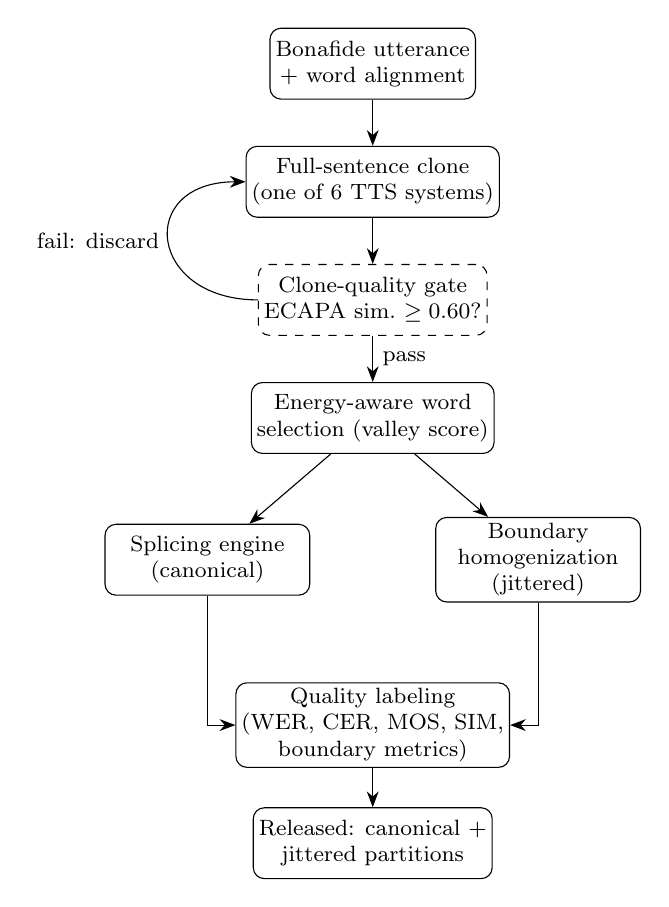
\begin{tikzpicture}[
  box/.style={draw, rounded corners, align=center, minimum width=2.6cm,
              minimum height=0.9cm, font=\footnotesize, inner sep=2pt},
  gate/.style={box, dashed},
  arr/.style={-{Stealth[length=2mm]}}
]
\node[box] (input) at (0,0) {Bonafide utterance\\+ word alignment};
\node[box] (clone) at (0,-1.5) {Full-sentence clone\\(one of 6 TTS systems)};
\node[gate] (gate) at (0,-3.0) {Clone-quality gate\\ECAPA sim.\ $\geq 0.60$?};
\node[box] (select) at (0,-4.5) {Energy-aware word\\selection (valley score)};
\node[box] (canon) at (-2.1,-6.3) {Splicing engine\\(canonical)};
\node[box] (jitter) at (2.1,-6.3) {Boundary\\homogenization\\(jittered)};
\node[box] (quality) at (0,-8.4) {Quality labeling\\(WER, CER, MOS, SIM,\\boundary metrics)};
\node[box] (output) at (0,-9.9) {Released: canonical +\\jittered partitions};

\draw[arr] (input) -- (clone);
\draw[arr] (clone) -- (gate);
\draw[arr] (gate) -- node[right,font=\footnotesize]{pass} (select);
\draw[arr] (gate.west) .. controls +(-1.4,0) and +(-1.4,0) ..
  node[left,font=\footnotesize]{fail: discard} (clone.west);
\draw[arr] (select) -- (canon);
\draw[arr] (select) -- (jitter);
\draw[arr] (canon.south) |- (quality.west);
\draw[arr] (jitter.south) |- (quality.east);
\draw[arr] (quality) -- (output);
\end{tikzpicture}
\caption{Partial-spoof pipeline overview. A failed clone-quality check
discards the clone as a generation failure rather than an attack; the
canonical and boundary-homogenized (jittered) branches are released as
separate sentence-disjoint partitions but pass through the same
quality-labeling stage.}
\label{fig:partialpipeline}
\end{figure}

\paragraph{Cloning and word extraction.} Rather than synthesizing each
replacement word in isolation, which yields flat and non-natural
prosody, the pipeline clones the \emph{full} sentence in the target voice
with one of the six previously described TTS systems, and extracts the
required words from the full synthesized utterance by word-level
alignment. Each bonafide file is dispatched to exactly one of the six
systems via a weighted random draw (40\% OmniVoice, 20\% Qwen3-TTS,
10\% each for the remaining four systems), rather than attacking every
file with every system; the weights were set empirically from informal
listening comparisons during development, favoring systems whose
output was judged harder to identify as synthetic, and were not
validated by a systematic evaluation. In-context words carry natural coarticulation and prosody,
making the splice harder to detect. Only utterances whose speaker
similarity to the target speaker is at least 0.60 proceed to splicing.
Below-threshold clones do not resemble the target and are discarded as
generation failures, excluded from the released attack counts.

\paragraph{Energy-aware word selection.} Candidate replacement words are
not chosen at random. The goal is to insert each spoofed word where it is
least audible, e.g., within pauses rather than in the middle of connected
speech. To find such regions, every word boundary $b$ in the cloned audio is
given a \emph{valley score} $s(b)$, computed from the clone's own
energy profile at the splice point rather than the original
recording's, which determines whether the insertion will be
audible. Let $W_b$ denote the set of
short-time analysis frames whose centers lie within $\pm 100$\,ms of the
boundary, let $N_b = |W_b|$ be the number of such frames, and let
$\mathrm{RMS}(t) \ge 0$ be the RMS energy of frame $t$ (frames are
5\,ms long, thus $N_b = 40$ away from the signal edges). The score is
\begin{equation}
s(b) \;=\; \frac{\displaystyle\min_{t \in W_b} \mathrm{RMS}(t)}
                 {\displaystyle\frac{1}{N_b}\sum_{t \in W_b} \mathrm{RMS}(t)}
\label{eq:valleyscore}
\end{equation}
That is, the quietest instant in the window divided by the window's
average loudness. Since RMS energy is non-negative and a minimum can
never exceed the corresponding mean, $s(b) \in [0,1]$ by construction. A
boundary that falls in clear inter-word silence has almost no energy at
its quietest instant, thus $s(b) \to 0$. A boundary buried in continuous
speech never quiets down within the window, thus $s(b) \to 1$. Each word
has two boundaries, left and right, each scored independently as
$s(b)$. For interior words the combined score is the maximum of the
two, since both cuts must be clean for the splice to be inaudible; for
the first and last word of the utterance, only the single internal
boundary counts, the other side being the sentence edge rather than a
cut. Only words whose combined score falls at or below 0.65, and whose
duration exceeds 200\,ms, are eligible for replacement. To validate
this choice, we swept the threshold over $\{0.3, 0.5, 0.65, 0.8, 1.0\}$
against the already-generated clones of all six attack systems. The
pattern is consistent. Threshold 0.65 already captures 94--98\% of the
selection-plan yield achievable with no filtering at all (OmniVoice
95.9\%, Qwen3-TTS 94.1\%, Chatterbox 98.1\%, Fish-Speech 98.4\%,
OuteTTS 98.1\%, OpenVoice 95.0\% on its much smaller $n=9$ aligned
sample). Raising the threshold further buys little additional yield
while admitting boundaries with progressively less energy dip; 0.65
was therefore retained as the production value. Eligible words are then selected
greedily, lowest combined score (quietest boundaries) first, subject to
a non-adjacency constraint (selected word indices differ by at least
two). This distributes the spoofed content across the utterance rather
than forming a single contiguous block that would resemble a
segment-level rather than a word-level attack.

Figure~\ref{fig:splicesteps}
shows the five steps the engine applies to each replacement. (1)~It
refines the Parakeet word timestamps by local energy analysis, correcting
the 100--\SI{300}{\milli\second} drift the transducer can exhibit on fast
connected speech. (2)~It snaps each cut outward to the nearest silence,
placing the seam at low energy. (3)~It inserts the cloned word at its
\emph{natural} duration, without time-stretching, preserving the clone's
pitch. (4)~It matches the cloned word's loudness to a voiced-RMS anchor
computed once from the bonafide host, removing loudness as a spoof cue.
(5)~It blends the seams with a crossfade bounded by the available silence
on each side, so that the fade does not bleed a neighboring word into the
splice.
Because TTS output typically packs consecutive words with little
inter-word silence, this bound is usually tighter than the nominal
$[30,80]$\,ms sampling range. When there is no silence at all on one
side (the next or previous word begins immediately, with no gap), the
crossfade on that side collapses entirely to a hard cut (0\,ms). The
released mean effective crossfade (3.9--4.9\,ms,
Table~\ref{tab:pstierquality}) reflects how often this happens. For
multi-word tiers, a running offset maps each subsequent cut onto the
current audio after earlier insertions have changed its
length.

\begin{figure}[t]
\centering
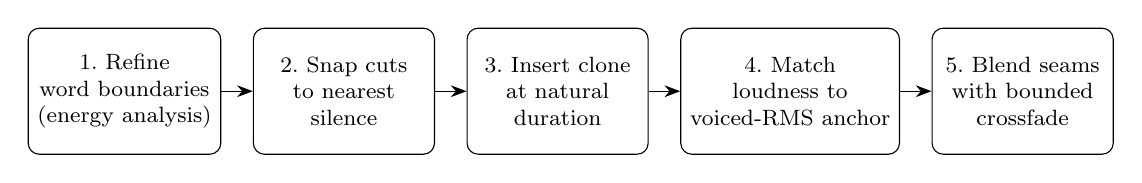
\begin{tikzpicture}[
  node distance=4mm,
  stepn/.style={draw, rounded corners, align=center, minimum width=2.3cm,
               minimum height=1.6cm, font=\footnotesize},
  arr/.style={-{Stealth[length=2mm]}}
]
\node[stepn] (s1) {1.\ Refine\\word boundaries\\(energy analysis)};
\node[stepn, right=of s1] (s2) {2.\ Snap cuts\\to nearest\\silence};
\node[stepn, right=of s2] (s3) {3.\ Insert clone\\at natural\\duration};
\node[stepn, right=of s3] (s4) {4.\ Match\\loudness to\\voiced-RMS anchor};
\node[stepn, right=of s4] (s5) {5.\ Blend seams\\with bounded\\crossfade};
\draw[arr] (s1) -- (s2);
\draw[arr] (s2) -- (s3);
\draw[arr] (s3) -- (s4);
\draw[arr] (s4) -- (s5);
\end{tikzpicture}
\caption{Five-step splicing engine applied to each word replacement.
Steps 1--2 place the seam. Step 3 preserves the clone's natural pitch by
avoiding time-stretching. Step 4 removes loudness as a possible spoof
cue. Step 5 smooths the seam within the available silence budget.}
\label{fig:splicesteps}
\end{figure}

For each splice, the engine draws the seam technique from
seven options in fixed proportions (Table~\ref{tab:splice}), ranging from
a hard cut to several equal-gain and equal-power fade laws. Randomizing
the seam prevents a detector from keying on a single fade signature. The
engine also draws one overlap duration per splice from a fixed range and
bounds it by the available silence.

\begin{table}[H]
\centering
\caption{Splice seam techniques and their sampling
proportions, as implemented. Fade-in curves are given for
$t\in[0,1]$; the fade-out is the time-reverse. Method~5 applies the
square-root (equal-power) law $\sqrt{t}$.}
\label{tab:splice}
\small
\begin{tabular}{clcc}
\toprule
\textbf{\#} & \textbf{Technique} & \textbf{Fade-in curve} & \textbf{Proportion} \\
\midrule
1 & Hard cut (no fade)          & ---                       & 10\% \\
2 & Overlap-add, Hann window    & $0.5(1-\cos\pi t)$        & 20\% \\
3 & Linear                      & $t$                       & 15\% \\
4 & Cosine (equal-power)        & $\sin(\pi t/2)$           & 20\% \\
5 & Square-root (equal-power)   & $\sqrt{t}$                & 15\% \\
6 & Logarithmic                 & $\log(1+9t)/\log 10$      & 10\% \\
7 & Inverted parabola           & $1-(1-t)^2$               & 10\% \\
\bottomrule
\end{tabular}
\end{table}

\paragraph{Boundary-homogenization variant.} A naive
partial spoof leaves only the two boundaries flanking the replaced word
anomalous; consequently, a detector can use the single discontinuous boundary as a
shortcut and achieve low error without learning any synthesis artifact
\citep{negroni2024splicing}. MARSA suppresses this shortcut with a
parallel \emph{jittered} variant of the partial-spoof tier. In this
variant, \emph{every} internal word boundary of an utterance, genuine or
spliced, independently undergoes, with probability 0.5, one of three
structural manipulations chosen uniformly. These manipulations differ
from the seven crossfade techniques of Table~\ref{tab:splice}, which
shape the splice seam itself:
\begin{enumerate}
  \item a short truncation of one word's edge
  (10--\SI{40}{\milli\second}, shorter than a Spanish syllable nucleus
  to preserve intelligibility);
  \item a Hann-windowed overlap of the two words
  (30--\SI{80}{\milli\second}, matching the crossfade range of prior
  partial-spoof work \citep{luong2024llama}); and
  \item a bleed of one word's edge into its neighbor
  (20--\SI{60}{\milli\second}, covering Spanish voice-onset time plus a
  consonant-vowel transition).
\end{enumerate}
A manipulation probability of 0.5 maximizes the entropy of
the ``manipulated or not'' signal at each boundary, which means the act of
manipulation no longer distinguishes the spliced boundary. MARSA releases
the jittered variant as a separate sentence-disjoint partition, so that
detectors can be trained and evaluated on the canonical and jittered
distributions independently or jointly.

\paragraph{Quality labeling without filtering.} The partial-spoof
generation pipeline computes WER, CER, a perceptual quality score,
speaker similarity, and boundary metrics for every sample, but does
\emph{not} discard low-quality samples. Each sample instead carries a
categorical \texttt{quality\_flag} (high/medium/low). Downstream users
may stratify or filter on it. Only structural failures (zero
successfully spliced words or missing or unreadable audio) are removed,
since those are not partial spoofs at all. This "keep-everything,
label-everything" policy reflects the fact that a real attacker does not
post-filter output, and a detector trained only on clean attacks may
collapse on noisy ones. The generated partial-spoof data are summarized
by system, replacement tier, boundary-jitter partition, and quality flag
in Tables~\ref{tab:pscompsystem} and \ref{tab:pscompbreakdown}
(Chapter~\ref{ch:data-records}).

\section{Acoustic Augmentation}
\label{sec:augmentation}

To support the study of channel robustness without regenerating attacks,
MARSA provides an augmentation layer that transforms the base corpus
into a channel-degraded training set. The layer is applied identically
to bonafide and spoof audio. The augmentation type, the augmentation
rate, and the output loudness are therefore all decoupled from the class
label. In particular, every file is loudness normalized by the same
policy; therefore, neither the presence of an augmentation nor its output level
is biased toward a specific class. Without this process, an
anti-spoofing model can learn "augmented implies one class" or "louder
implies one class" and collapse at evaluation time on clean, uniformly
scaled audio.

\paragraph{Copies per file.} For each original training file, the
augmentation layer emits one clean copy plus a number of augmented
copies set by the corpus-multiplication factor. At the smallest factor
roughly one half of the training set stays clean; larger factors lower
that fraction. The development and evaluation splits are released at
factor one and are never augmented; model selection and testing therefore occur
on clean audio.

\paragraph{Augmentation mode.} For each augmented clip, a
random draw selects the mode. With probability 0.6, the layer applies a
single augmentation, choosing between reverberation-plus-noise and codec
degradation in a 60:40 ratio. With probability 0.4, it \emph{stacks} the
two: reverberation and noise first, then a codec round-trip on the
result. Stacking simulates the common case of a reverberant, noisy source
transmitted over a lossy channel. The sample's system identifier records
the augmentation chain, with a pipe separator for stacked clips (for
example \texttt{RIR\_SMALL\_NOI\_SNR15|CODEC\_OPUS\_LOSS3PCT}); the full
history is therefore recoverable from the protocol file without restructuring
directories. We release the augmentation at four multiplication factors
($\times$2, $\times$3, $\times$5, $\times$10), each applied equally to
bonafide and spoof audio. The clean fraction is therefore identical
across classes, and augmentation does not shift the class balance. We
leave rebalancing of the spoof-heavy corpus to the user at training time
(Chapter~\ref{ch:discussion}), which keeps augmentation from becoming a
class cue.

\paragraph{Reverberation and noise.} This family
convolves the clip with a room impulse response from the RIRS\_NOISES set
\citep{ko2017rir}, stratified into small, medium, and large rooms
(sampled at 30\%, 50\%, and 20\%), and then adds noise from MUSAN
\citep{musan}. The noise source is ambient noise, multi-speaker babble, or
music (sampled at 50\%, 30\%, and 20\%), mixed at a signal-to-noise ratio
(SNR) drawn from three bands (0--5\,dB, 5--30\,dB, and 30--35\,dB)
weighted 10\%, 80\%, and 10\%. Most clips therefore show moderate
degradation, with a light tail at each extreme.

\paragraph{Codec degradation.} This family applies a real
encode-then-decode round-trip through six telephony and VoIP codecs that
represent the target deployment channels: G.711 $\mu$-law and A-law (PSTN
and landline), AMR-NB (2G/3G mobile), Speex (legacy VoIP), Opus (the
dominant over-the-top codec in consumer messaging and conferencing apps),
and AAC (broadband). For codecs with a selectable bitrate, the layer
draws a bitrate from the encoder's supported set; with a fixed
probability, it also simulates packet loss at a sampled loss fraction.
The signal is resampled to each codec's native rate for the round-trip
and back to \SI{16}{\kilo\hertz} on write. All six codecs appear in the
released corpus, each within 0.2 percentage points of its target mix
weight (Chapter~\ref{ch:evaluation}). We chose this codec set for
deployment realism. A broader design with wideband and enterprise codecs,
a burst-loss channel model, and per-codec packet-loss concealment is a
planned extension and is not part of the released corpus.

\paragraph{Training-time augmentation.} A convolutive and
additive signal-level augmentation of the RawBoost family
\citep{tak2022ssl} is meant to be applied on the fly during detector
training. Because this fast, waveform-level operation gains nothing from
precomputation, we document it here and provide it in the accompanying
code, but it is not part of the deposited files.

\section{Parameter Summary}
\label{sec:params}

Tables~\ref{tab:params-fullspoof}--\ref{tab:params-quality}
list the numeric parameters that govern generation, grouped by pipeline
stage; the released code and these values suffice to regenerate the
corpus. A fixed base seed (42) combined with a per-sample key hash drives
every stochastic choice; the assignment of attack systems, word
selections, splice techniques, and jitter plans is therefore deterministic and
reproducible across runs. Distributions are written as
value~(probability); intervals sampled uniformly are written
Uniform$[a,b]$.

\begin{table}[H]
\centering
\caption{Key generation parameters: full-spoof screening.}
\label{tab:params-fullspoof}
\small
\begin{tabular}{p{4.9cm}p{7.2cm}}
\toprule
\textbf{Parameter} & \textbf{Value} \\
\midrule
WER rejection threshold & 0.15 (hard gate) \\
CER rejection threshold & 0.10 (hard gate) \\
NISQA MOS, speaker similarity & recorded for reference only; no rejection gate applied \\
Regeneration budget & up to 5 rounds on structural or intelligibility failure \\
\bottomrule
\end{tabular}
\end{table}

\begin{table}[H]
\centering
\caption{Key generation parameters: partial-spoof word selection.}
\label{tab:params-wordselect}
\small
\begin{tabular}{p{4.9cm}p{7.2cm}}
\toprule
\textbf{Parameter} & \textbf{Value} \\
\midrule
Tier minimum sentence length & W1: 4, W2: 8, W3: 12 words \\
Non-adjacency constraint & selected word indices differ by $\geq 2$ \\
Valley-score window / frame & $\pm$\SI{100}{\milli\second} / \SI{5}{\milli\second} \\
Valley-score eligibility & combined score $\leq 0.65$ \\
Minimum word duration & \SI{200}{\milli\second} \\
Clone acceptance gate & Speaker similarity $\geq 0.60$ \\
\bottomrule
\end{tabular}
\end{table}

\begin{table}[H]
\centering
\caption{Key generation parameters: partial-spoof splice engine.}
\label{tab:params-splice}
\small
\begin{tabular}{p{4.9cm}p{7.2cm}}
\toprule
\textbf{Parameter} & \textbf{Value} \\
\midrule
Energy-refinement radius & \SI{300}{\milli\second} \\
Silence RMS threshold & 0.015 (of full scale) \\
Valley-snap search half-width & \SI{50}{\milli\second} \\
Crossfade overlap & Uniform$[30,80]$~ms, clamped to the inter-word gap \\
Splice-technique proportions & see Table~\ref{tab:splice} \\
Loudness match & per-utterance voiced-RMS anchor; frame \SI{20}{\milli\second}; voiced gate $0.15\times$P95; peak threshold 0.99 \\
\bottomrule
\end{tabular}
\end{table}

\begin{table}[H]
\centering
\caption{Key generation parameters: boundary-jitter variant.}
\label{tab:params-jitter}
\small
\begin{tabular}{p{4.9cm}p{7.2cm}}
\toprule
\textbf{Parameter} & \textbf{Value} \\
\midrule
Per-boundary manipulation probability & 0.50 \\
Truncate / overlap / bleed range & Uniform$[10,40]$ / $[30,80]$ / $[20,60]$~ms \\
\bottomrule
\end{tabular}
\end{table}

\begin{table}[H]
\centering
\caption{Key generation parameters: acoustic augmentation.}
\label{tab:params-augmentation}
\small
\begin{tabular}{p{4.9cm}p{7.2cm}}
\toprule
\textbf{Parameter} & \textbf{Value} \\
\midrule
Family mix & RIR+noise 0.60, codec 0.40 \\
Stacking-gate probability & 0.40 (RIR+noise then codec) \\
Room size & small 0.30, medium 0.50, large 0.20 \\
Noise source & noise 0.50, babble 0.30, music 0.20 \\
SNR band (dB) & $[0,5]$ (0.10), $[5,30]$ (0.80), $[30,35]$ (0.10) \\
Codec weights & G.711$\mu$ 0.25, G.711A 0.15, AMR-NB 0.20, Speex 0.05, Opus 0.25, AAC 0.10 \\
Codec bitrates (kbps) & AMR-NB $\{4.75\text{--}12.2\}$; Opus $\{8,12,16,24,32\}$; AAC $\{24,32,48,64\}$; G.711/Speex fixed \\
Packet loss & applied with prob.\ 0.30; fraction Uniform$[0,0.05]$ \\
Multiplication factors & $\times$2, $\times$3, $\times$5, $\times$10; same factor applied to both classes \\
\bottomrule
\end{tabular}
\end{table}

\begin{table}[H]
\centering
\caption{Key generation parameters: quality-flag thresholds (partial spoof).}
\label{tab:params-quality}
\small
\begin{tabular}{p{4.9cm}p{7.2cm}}
\toprule
\textbf{Parameter} & \textbf{Value} \\
\midrule
high & WER $\leq 0.10$, NISQA MOS $\geq 4.0$, spk. similarity $\geq 0.50$ \\
medium & WER $\leq 0.30$ (and not high) \\
low & otherwise \\
\bottomrule
\end{tabular}
\end{table}

% =====================================================================
\chapter{Corpus Description}
\label{ch:data-records}

The corpus is deposited in the Zenodo open repository
under a single versioned record (DOI: \url{https://doi.org/10.5281/zenodo.23873176}).

The release mirrors the ASVspoof2019 LA convention; common
anti-spoofing training and evaluation libraries therefore read it directly.
Each tier is a flat directory of FLAC audio files with a protocol text
file. Each protocol line names the speaker, the utterance identifier, the
system identifier, and the class label:

\begin{quote}\small
\texttt{arf\_00295\ LA\_T\_12000000\ FISHGRAM\_PSW1\ partial\_spoof}
\end{quote}

Class labels are \texttt{bonafide}, \texttt{spoof}, and
\texttt{partial\_spoof}. System identifiers encode the generating system
and, for partial spoof, the tier: \texttt{PSW1}/\texttt{PSW2}/%
\texttt{PSW3} for one/two/three replaced words, with a trailing
\texttt{J} for the boundary-homogenized (jittered) variant. Utterance
identifiers are assigned in disjoint numeric ranges per tier and
variant; they never collide across the corpus. For the partial-spoof
tier, a companion table lists, for every spoofed word, its start and end
time within the audio and the splice technique used. These constitute
the frame-level spoof labels. Per-sample metadata (the acoustic-quality
metrics and \texttt{quality\_flag} described in
Chapter~\ref{ch:methods}) are provided as CSV tables aggregated across
all pipelines.

The full-spoof tier's content, by generating system, is given in
Table~\ref{tab:fullspoofdesc}. Utterance counts differ by system
(25{,}642--34{,}197) because each system targets a 1:1 generation ratio
against the 35{,}927 bonafide utterances, but the realized count
reflects its individual pass rate through the quality gate
(Section~\ref{sec:fullspoof}).

\begin{table}[H]
\centering
\caption{Generated full spoof content, detailed by
TTS system. \textbf{Duration} and \textbf{Words} describe the
duration (in seconds) of the generated audio and its Common Voice target text, respectively. \textbf{Hours} refers to total generated-audio duration.}
\label{tab:fullspoofdesc}
\small
\begin{tabular}{lrccc}
\toprule
\textbf{System} & \textbf{Utterances} & \textbf{Duration ($\sigma$)}  & \textbf{Words ($\sigma$)} & \textbf{Hours} \\
\midrule
Fish-Speech & 34{,}197 & 3.80 (1.05) & 10.4 (2.6) & 36.1 \\
Qwen3-TTS              & 31{,}568 & 4.57 (1.22) & 10.4 (2.6) & 40.1 \\
OpenVoice v2           & 29{,}796 & 4.52 (0.98) & 10.4 (2.6) & 37.5 \\
Chatterbox             & 31{,}701 & 3.96 (1.13) & 10.4 (2.6) & 34.8 \\
OuteTTS                & 25{,}642 & 4.33 (1.11) & 10.4 (2.6) & 30.9 \\
OmniVoice              & 33{,}743 & 4.19 (1.38) & 10.3 (2.6) & 39.3 \\
\midrule
\textbf{Total}         & \textbf{186{,}647} & 4.22 (1.19) & 10.4 (2.6) & \textbf{218.6} \\
\bottomrule
\end{tabular}
\end{table}

The composition of the partial-spoof tier is given in
Tables~\ref{tab:pscompsystem} and \ref{tab:pscompbreakdown}.

\begin{table}[H]
\centering
\caption{Partial-spoof tier composition by generating system
(18{,}421 spliced utterances total).}
\label{tab:pscompsystem}
\small
\begin{tabular}{lr}
\toprule
\textbf{System} & \textbf{Count} \\
\midrule
OmniVoice   & 10{,}990 \\
Qwen3-TTS   &  1{,}565 \\
Chatterbox  &  3{,}423 \\
Fish-Speech &  1{,}317 \\
OuteTTS     &  1{,}073 \\
OpenVoice   &     53   \\
\midrule
\textbf{Total} & \textbf{18{,}421} \\
\bottomrule
\end{tabular}
\end{table}

\begin{table}[H]
\centering
\caption{The same 18{,}421 partial-spoof utterances, broken down
independently by replacement tier, boundary-jitter partition, and
quality flag. These are three separate groupings of the same total,
not a further split of Table~\ref{tab:pscompsystem}'s per-system
counts.}
\label{tab:pscompbreakdown}
\small
\begin{tabular}{lr}
\toprule
\textbf{Grouping} & \textbf{Count} \\
\midrule
\multicolumn{2}{l}{\emph{Replacement tier}} \\
\quad W1 (1 word)  & 10{,}276 \\
\quad W2 (2 words) &  5{,}991 \\
\quad W3 (3 words) &  2{,}154 \\
\addlinespace
\multicolumn{2}{l}{\emph{Boundary-jitter partition}} \\
\quad canonical  &  8{,}456 \\
\quad jittered   &  9{,}965 \\
\addlinespace
\multicolumn{2}{l}{\emph{Quality flag}} \\
\quad high   &  4{,}875 \\
\quad medium & 13{,}072 \\
\quad low    &    474 \\
\bottomrule
\end{tabular}
\end{table}

Each bonafide file is dispatched to exactly one TTS system by weighted
draw (Section~\ref{sec:partialspoof}), but the realized per-system
composition diverges substantially from those dispatch weights.
Survival through the downstream clone-similarity gate and
word-eligibility filtering ranges from 1.5\% (OpenVoice, mean
full-spoof similarity 0.388) to 97.2\% (Chatterbox). This survival rate
does not track full-spoof speaker similarity in a simple way:
Qwen3-TTS has the highest mean full-spoof similarity of the six
systems (0.720) yet only a 22.3\% survival rate, while Chatterbox,
with nearly identical similarity (0.714), survives at 97.2\%. The
dispatch stage itself is correctly calibrated (realized weights within
one percentage point of target for every system); the divergence
originates downstream, in a mechanism this corpus does not fully
isolate. The tier's per-system composition is therefore narrower than
that of the full-spoof tier. The
corpus is dominated by the W1 tier because most eligible utterances are
short enough to admit only a single replacement. All 18{,}421 samples are
released, unfiltered by quality. The recommended clean partition is
identifiable directly from the released per-sample metrics
(Chapter~\ref{ch:evaluation}; see also Chapter~\ref{ch:discussion}).

The augmentation tiers use the same protocol convention
and record the augmentation chain in the system identifier field
(Section~\ref{sec:augmentation}).

The deposited record (\texttt{MARSA\_augmented\_2x.zip}),
approximately 29\,GB, has the following structure:

\begin{quote}\small
\begin{verbatim}
MARSA_augmented_2x.zip
  augmented_2x/LA/
    MARSA_LA_train/
      flac/                                  (FLAC audio)
      MARSA.LA.cm.train.trn.txt              (protocol)
      MARSA.LA.cm.train.metadata.csv         (augmentation metadata)
    MARSA_LA_dev/
      flac/
      MARSA.LA.cm.dev.trl.txt
      MARSA.LA.cm.dev.metadata.csv
    MARSA_LA_eval/
      flac/
      MARSA.LA.cm.eval.trl.txt
      MARSA.LA.cm.eval.metadata.csv
\end{verbatim}
\end{quote}

\section{Code Availability}

The full generation pipeline (the six full-spoof attack systems'
wrappers, the partial-spoof splicing engine, the boundary-jitter
variant, and the augmentation layer) is publicly available at
\url{https://github.com/Tomas1307/ANTI-SPOOFING-VOICE-LATIN-AMERICA},
released as open-source software under the Apache License 2.0, with
the exact configuration and random seeds used to produce the released
corpus pinned in each pipeline's settings module. The pipeline is
implemented in Python and orchestrated to make each tier reproducible
from the bonafide source. The codec-degradation family
(Section~\ref{sec:augmentation}) requires a static ffmpeg build with
AMR-NB and AAC encoding support (a stock system ffmpeg typically lacks
both). The repository includes a checksum-verified script that fetches
the exact pinned ffmpeg build used to generate the released corpus,
rather than assuming an equivalent build is already present on the
host system.

\section{Data Availability}

All MARSA audio, protocol files,
frame-level label tables, and per-sample metadata are openly available
from the Zenodo record cited above. The bonafide source recordings
derive from HABLA \citep{habla}; users who need the original
unprocessed bonafide audio should consult that resource.

% =====================================================================
\chapter{Evaluation}
\label{ch:evaluation}

Two forms of evidence establish that MARSA is fit for
purpose: the intrinsic quality of the generated audio and its extrinsic
usefulness for anti-spoofing detection.

\section{Intrinsic Quality of Generated Attacks}

We screened every generated utterance for
intelligibility, perceptual quality, and speaker fidelity with three
metrics computed during generation (Chapter~\ref{ch:methods}). WER
compares a Parakeet transcription of the generated audio with the target
text. Perceptual quality is the mean opinion score (MOS) predicted by the
NISQA speech-quality model \citep{nisqa}; of the five NISQA dimensions
(overall MOS, noisiness, discontinuity, coloration, and loudness), we use
only the overall MOS. Speaker fidelity is the cosine similarity between
ECAPA-TDNN speaker embeddings of the generated audio and the target
speaker \citep{ecapa}, the same measure used to de-duplicate speakers
between HABLA and Common Voice
(Section~\ref{sec:bonafide}).
Table~\ref{tab:fullspoof} reports the mean full-spoof screening
metrics.

\begin{table}[H]
\centering
\caption{Quality assessment of the full spoof data.
WER and CER are word- and character-error rate against the target
text. MOS is the overall mean opinion score predicted by the NISQA speech-quality model \citep{nisqa} (1--5, higher better). SIM
is ECAPA-TDNN cosine speaker similarity to the source audio (higher better).}
\label{tab:fullspoof}
\small
\begin{tabular}{lrcccc}
\toprule
\textbf{System} & \textbf{Utterances} & \textbf{WER (\%)} & \textbf{CER (\%)} & \textbf{MOS} & \textbf{SIM} \\
\midrule
Fish-Speech & 34{,}197 & 2.17 & 0.70 & 4.57 & 0.602 \\
Qwen3-TTS              & 31{,}568 & 1.46 & 0.59 & 4.37 & 0.720 \\
OpenVoice v2           & 29{,}796 & 1.50 & 0.45 & 4.38 & 0.388 \\
Chatterbox             & 31{,}701 & 1.20 & 0.34 & 4.39 & 0.714 \\
OuteTTS                & 25{,}642 & 2.36 & 0.85 & 4.45 & 0.462 \\
OmniVoice              & 33{,}743 & 1.06 & 0.30 & 4.28 & 0.686 \\
\midrule
\textbf{Total}         & \textbf{186{,}647} & & & & \\
\bottomrule
\end{tabular}
\end{table}

The systems differ deliberately while keeping the identity of the
source speaker. Speaker similarity spans a wide band, from 0.388
(OpenVoice, whose tone-conversion architecture lets the synthesis base
voice bleed through) through 0.462 (OuteTTS) and the high-fidelity
cluster of Qwen3-TTS (0.720), Chatterbox (0.714), and OmniVoice
(0.686). Perceptual quality (NISQA MOS) is uniformly high, from 4.28 to
4.57, and WER is at or below 2.4\% for every system. This spread is
deliberate. An anti-spoofing model trained on MARSA will cover both
high-fidelity and low-fidelity attacks rather than a single narrow band
of synthesis quality, and these results confirm that the attacks are
intelligible, natural-sounding, and (for the stronger systems) close to
the target speaker, that is, credible spoofing attempts rather than
degenerate synthesis.

For the partial-spoof tier, quality metrics are computed per sample and
released as labels rather than used as filters. The corpus therefore
spans the full realistic quality range; under the resulting
\texttt{quality\_flag} the 18{,}421 spliced samples divide into 4{,}875
high, 13{,}072 medium, and 474 low, and 15{,}641 (84.9\%) pass the
full-spoof intelligibility gate (WER $\leq 0.15$, CER $\leq 0.10$) that
defines the recommended clean partition. These are independent
criteria. \texttt{quality\_flag} additionally weighs NISQA
and speaker similarity (Table~\ref{tab:params-quality}); a sample's
flag and its clean-partition membership need not agree. Of the 2{,}780
samples that fail the clean partition, 474 are flagged low (all of
them, since low requires WER $>0.30$), 2{,}265 are flagged medium
(whose WER $\leq 0.30$ band straddles the clean partition's 0.15
cutoff), and 41 are flagged high despite WER $\leq 0.10$, failing only
on the independent CER $\leq 0.10$ criterion.
Table~\ref{tab:pstierquality}
reports WER, CER, MOS score, and speaker similarity broken down by
replacement tier, computed over the released per-sample metrics.

\begin{table}[H]
\centering
\caption{Quality assessment of the partial spoof data by replacement tier. WER and CER are against the target
transcript. MOS is the no-reference perceptual-quality score. SIM is
ECAPA-TDNN cosine similarity between the spliced result and the target
speaker; it is naturally higher than full-spoof SIM (Table~\ref{tab:fullspoof})
since most of a partial-spoof utterance is genuine audio. Crossfade: mean duration actually applied at each seam
(Section~\ref{sec:partialspoof}). This is usually much shorter than
the nominal $[30,80]$\,ms range the engine samples from, because the
TTS clone rarely has that much silence next to the spliced word.}
\label{tab:pstierquality}
\small
\begin{tabular}{lrccccc}
\toprule
\textbf{Tier} & \textbf{Utt.} & \textbf{WER (\%)} & \textbf{CER (\%)} & \textbf{MOS} & \textbf{SIM} & \textbf{Crossfade (ms)} \\
\midrule
W1 (1 word)  & 10{,}276 & 4.61 & 2.36 & 3.53 & 0.781 & 4.87 \\
W2 (2 words) &  5{,}991 & 6.08 & 3.25 & 3.28 & 0.799 & 4.31 \\
W3 (3 words) &  2{,}154 & 6.80 & 3.74 & 3.14 & 0.820 & 3.89 \\
\midrule
\textbf{Total} & \textbf{18{,}421} & 5.34 & 2.81 & 3.40 & 0.791 & 4.41 \\
\bottomrule
\end{tabular}
\end{table}

MOS runs lower in the partial-spoof tier (3.14--3.53 across
replacement tiers, Table~\ref{tab:pstierquality}) than in full-spoof
(4.28--4.57, Table~\ref{tab:fullspoof}), the opposite direction from
SIM. A full-spoof utterance is internally coherent, generated in a
single synthesis pass, whereas a partial-spoof utterance joins genuine
and cloned audio at a splice boundary. The crossfade actually applied
there is short (3.9--4.9\,ms mean, well under the engine's
$[30,80]$\,ms target range, Table~\ref{tab:pstierquality}), and even a
short discontinuity in spectral content or background noise across
that seam is enough for a no-reference quality model to penalize the
whole utterance, despite most of the signal being genuine. This is
consistent with the same splice-boundary artifact that motivates the
boundary-jitter variant and the prior forensic finding that
discontinuous boundaries, not synthesis quality, are what a naive
detector can exploit \citep{negroni2024splicing,huang2024detectable}.

Table~\ref{tab:pssystemquality} breaks down the same
per-sample metrics by generating system and is the partial-spoof
counterpart of Table~\ref{tab:fullspoof}.

\begin{table}[H]
\centering
\caption{Quality assessment of the partial spoof data by generating
system. Columns follow Table~\ref{tab:pstierquality}; systems are
ordered as in Table~\ref{tab:fullspoof} for direct comparison across
the full-spoof and partial-spoof tiers.}
\label{tab:pssystemquality}
\small
\begin{tabular}{lrcccc}
\toprule
\textbf{System} & \textbf{Utt.} & \textbf{WER (\%)} & \textbf{CER (\%)} & \textbf{MOS} & \textbf{SIM} \\
\midrule
Fish-Speech & 1{,}317  & 6.03 & 3.12 & 3.39 & 0.863 \\
Qwen3-TTS               & 1{,}565  & 4.62 & 2.37 & 3.32 & 0.850 \\
OpenVoice v2            &    53   & 3.49 & 1.50 & 3.09 & 0.898 \\
Chatterbox              & 3{,}423  & 5.85 & 3.17 & 3.40 & 0.807 \\
OuteTTS                 & 1{,}073  & 4.70 & 2.38 & 3.35 & 0.869 \\
OmniVoice               & 10{,}990 & 5.27 & 2.77 & 3.42 & 0.762 \\
\midrule
\textbf{Total}          & \textbf{18{,}421} & 5.34 & 2.81 & 3.40 & 0.791 \\
\bottomrule
\end{tabular}
\end{table}

OpenVoice shows the highest partial-spoof SIM (0.898),
although it is by far the weakest full-spoof cloner (0.388,
Table~\ref{tab:fullspoof}). This difference reflects a selection effect.
Only 53 OpenVoice clones clear the 0.60 ECAPA gate that admits a clone
into the partial-spoof tier (Section~\ref{sec:partialspoof}); the
surviving samples are therefore its best clones by construction, a
direct consequence of the gate rather than a representative picture of
its typical output.

\section{Bonafide Transcription Reliability}

Parakeet TDT is used for two distinct purposes in the pipeline, and
only one of them concerns the bonafide utterances directly. First,
every individual bonafide utterance is transcribed once
(Section~\ref{sec:bonafide}). This per-utterance transcript is not used
by full-spoof at all, but it is load-bearing for partial-spoof, where
it supplies both the text handed to the cloning system and the
word-level timestamps used for splice alignment, because partial-spoof
requires timing information tied to the exact bonafide recording being
edited, which no external transcript can supply
(Section~\ref{sec:partialspoof}). Second, Parakeet is run again,
separately, on each speaker's \emph{concatenated reference clip},
purely to give the full-spoof systems that use one a text hint
describing what that reference clip says. The content a full-spoof
system is actually asked to synthesize is independent of both of these
transcription steps. It is drawn directly from the original Common
Voice sentence rather than from any ASR output (Section~\ref{sec:fullspoof}).

The accuracy of the first of these, the per-utterance transcription
stage that partial-spoof depends on, was validated against an
independent ground truth. For the Common-Voice-origin bonafide subset,
where Common Voice's own original sentence serves as that ground truth,
it was compared to Parakeet's transcript of the same audio.
Table~\ref{tab:parakeetwer} reports WER and CER overall and per accent.
Overall WER is 3.02\% and CER is 0.87\%, consistent with Parakeet TDT's
published Spanish performance \citep{parakeet}. These results indicate
that the word-level timestamps underlying the partial-spoof tier are
anchored to a transcription stage with error rates in line with
expectations for the ASR model, rather than to unvalidated output.

\begin{table}[H]
\centering
\caption{Parakeet TDT transcription accuracy against original Common
Voice ground-truth sentences, for the Common-Voice-origin bonafide
subset. Venezuelan is shown for completeness but excluded from the
Overall row and from per-accent conclusions, since only one Venezuelan
speaker passed the Common Voice speaker-similarity filter
(Section~\ref{sec:bonafide}), leaving $n=4$, too few for a reliable
estimate.}
\label{tab:parakeetwer}
\small
\begin{tabular}{lrcc}
\toprule
\textbf{Accent} & \textbf{n} & \textbf{WER (\%)} & \textbf{CER (\%)} \\
\midrule
Chilean       &  1{,}247 & 1.93 & 0.48 \\
Peninsular    &  5{,}109 & 2.54 & 0.66 \\
Colombian     &    791 & 3.02 & 0.84 \\
Mexican       &  5{,}264 & 3.74 & 1.18 \\
Venezuelan ($n{=}4$) &   4 & 8.33 & 1.61 \\
\midrule
\textbf{Overall} & \textbf{12{,}411} & \textbf{3.02} & \textbf{0.87} \\
\bottomrule
\end{tabular}
\end{table}

\section{Augmentation Fidelity}

We verified the realized codec mix of the augmented corpus
against its configured target weights (Section~\ref{sec:params}).
Table~\ref{tab:codecfidelity} reports the target and realized proportion
of each codec. The largest gap is 0.2 percentage points (G.711
$\mu$-law); every other codec lies within 0.1 percentage points of its
target. A spectral check also confirmed that AMR-NB and Speex, the two
narrowband codecs in the mix, carry no energy above \SI{4}{\kilo\hertz},
consistent with their native bandwidth. The codec round-trip therefore
degrades the signal as intended.

\begin{table}[H]
\centering
\caption{Realized versus configured codec mix weights on the released
corpus (Section~\ref{sec:params} lists the configured targets).}
\label{tab:codecfidelity}
\small
\begin{tabular}{lrrr}
\toprule
\textbf{Codec} & \textbf{Target (\%)} & \textbf{Realized (\%)} & \textbf{Gap (pp)} \\
\midrule
G.711 $\mu$-law & 25.0 & 24.8 & $-0.2$ \\
G.711 A-law     & 15.0 & 14.9 & $-0.1$ \\
AMR-NB          & 20.0 & 20.1 & $+0.1$ \\
Speex           &  5.0 &  5.1 & $+0.1$ \\
Opus            & 25.0 & 24.9 & $-0.1$ \\
AAC             & 10.0 & 10.1 & $+0.1$ \\
\bottomrule
\end{tabular}
\end{table}

\section{Baseline Anti-spoofing Detection}
\label{sec:baseline}

Rather than train a new detector from scratch, this validation relies
on a sharper question: how do anti-spoofing models that already exist
perform when confronted with MARSA's attacks, without ever having seen
them? Four checkpoints are evaluated in a zero-shot setting. DF-Arena is
a 1.15-billion-parameter self-supervised detector, built from a
wav2vec\,2.0-XLS-R backbone \citep{babu2022xlsr} with a conformer
classification head, released on Hugging Face under the
Speech-Arena-2025 organization behind the Speech DF Arena leaderboard
\citep{dowerah2025speechdfarena}. Its backbone's self-supervised
pretraining is multilingual and includes Spanish among its 128
pretraining languages. No published source states this specific
checkpoint's own anti-spoofing training data directly. The closest
documented proxy is a related paper from the same research group, which
describes a training recipe explicitly built to follow the Speech DF
Arena approach: ASVspoof2019, ASVspoof2024, CodecFake, LibriSeVoc,
DFADD, CTRSVDD, SpoofCeleb, MLAAD, and EnvSDD \citep{raptor2026}. Of
these nine, only MLAAD includes Spanish, at a single accent out of its
54 languages; the remaining eight are English or Chinese. None of the
nine include any of MARSA's six TTS systems, all released in 2024 or
later. Whatever this checkpoint saw during anti-spoofing fine-tuning,
it did not see MARSA, and at most a thin, single-accent slice of
Spanish through MLAAD, nothing resembling the seven-accent,
cross-continental design this corpus targets. The other three models
correspond to LFCC-LCNN detectors with P2SGrad loss
\citep{wang2021comparative}, differing only in their pooling back-end
(LSTM-sum, fixed-length trim/pad, and self-attention), trained by a
collaborating group on an earlier, Spanish-only voice-cloning corpus
that predates MARSA and shares none of its six attack systems.

All four are evaluated using the $\times$2 augmentation tier's
speaker-disjoint development (30{,}808 clips, 155 speakers) and
evaluation (27{,}808 clips, 155 speakers) splits (never augmented,
regardless of tier), with zero speaker overlap against the training
partition. The dev and eval splits each contain exactly 155 speakers,
but the specific speakers assigned to each carry different numbers of
bonafide recordings (4{,}659 in dev vs.\ 4{,}072 in eval, consistent
with the corpus's per-speaker utterance imbalance,
Section~\ref{sec:bonafide}); this difference propagates through
full-spoof cloning and the $\times$2 augmentation factor to the
observed 30{,}808 vs.\ 27{,}808 total clip counts. DF-Arena's own feature
extractor requires an input of exactly \SI{4.0375}{\second} (64{,}600
samples). It truncates a longer clip to a centered window of that
length and tiles a shorter clip to fill it. The three LCNN detectors
carry no such requirement on their own and could in principle score
each clip in full. Applying DF-Arena's fixed window to all four
detectors instead, rather than letting the LCNN models see more of the
clip than DF-Arena does, keeps the input every detector receives
identical. A difference in EER across detectors then reflects a
difference in the detectors themselves, since every detector was
allowed to see the same amount of each clip. Table~\ref{tab:baseline} reports pooled Equal
Error Rate (EER, every clip) and strict EER (restricted to test clips
whose source sentence does not appear in training, joined via
\texttt{source\_file}) for both splits.

\begin{table}[H]
\centering
\caption{Zero-shot cross-corpus EER of four existing anti-spoofing detectors against
MARSA, $\times$2 augmentation tier. None of the four checkpoints was
trained on MARSA. Strict EER for a zero-shot model does not measure
train/test leakage; it only changes the test population toward
sentences absent from MARSA's own training split, a population that is
enriched toward full-spoof clips for these splits.}
\label{tab:baseline}
\small
\begin{tabular}{lcccc}
\toprule
\textbf{Model} & \textbf{Dev. pooled} & \textbf{Dev. strict} & \textbf{Eval pooled} & \textbf{Eval strict} \\
\midrule
DF-Arena \citep{dowerah2025speechdfarena} & 10.665\% & 8.510\% & 10.166\% & 8.001\% \\
LCNN self-attention \citep{wang2021comparative} & 24.620\% & 46.259\% & 18.761\% & 42.282\% \\
LCNN fixed-crop \citep{wang2021comparative} & 32.797\% & 44.341\% & 28.093\% & 43.053\% \\
LCNN LSTM-sum \citep{wang2021comparative} & 45.826\% & 56.151\% & 41.208\% & 60.749\% \\
\bottomrule
\end{tabular}
\end{table}

Two patterns emerge from the results. First, the modern self-supervised
detector generalizes far better than the classical hand-crafted-feature
family. DF-Arena's eval EER (10.166\%) highly outperforms the best LCNN
variant's (18.761\%), despite no confirmed exposure to Spanish
anti-spoofing data beyond, at most, MLAAD's single-accent slice, and no
exposure at all to any of these six TTS systems during training.
Despite the superior performance of the DF-Arena-based model, the
results are still far from what is required for a secure
production-ready SASV or anti-spoofing system.

Second, regarding the LCNN back-ends, self-attention pooling was the
strongest of the three architectures on its own matched Spanish test
set, and it remains the strongest here on pooled EER for both splits
and on eval strict EER; on dev strict EER, fixed-crop narrowly
outperforms it (44.341\% vs.\ 46.259\%). LSTM-sum is weakest throughout.
Because both the original training
data and MARSA are Spanish, this ranking survives a collapse in
absolute performance driven by a mismatch in TTS generation era rather
than by a language-transfer confound.

Table~\ref{tab:fullspoofeer} reports per-attack full-spoof EER for
DF-Arena on eval. OpenVoice and OuteTTS, the two weakest cloners by
speaker similarity (Table~\ref{tab:fullspoof}), are also the easiest
to detect (EER 0.027\% and 0.412\%). Qwen3-TTS, with the highest
speaker similarity (0.720), is a clear outlier at the opposite end
(18.046\%), nearly five times the next-highest system. Between these
extremes, the ordering is not strictly monotonic in similarity:
Chatterbox (SIM 0.714, nearly as high as Qwen) has one of the lowest
EERs (1.840\%), below Fish-Speech (SIM 0.602, EER 3.631\%) and
OmniVoice (SIM 0.686, EER 3.958\%). Attack realism therefore predicts
detectability at the extremes but not as a strict monotonic
relationship across all six systems.

\begin{table}[H]
\centering
\caption{Per-attack full-spoof EER for DF-Arena on the eval split,
with the corresponding ECAPA-TDNN speaker similarity from
Table~\ref{tab:fullspoof}.}
\label{tab:fullspoofeer}
\small
\begin{tabular}{lrr}
\toprule
\textbf{System} & \textbf{EER (\%)} & \textbf{SIM} \\
\midrule
OpenVoice v2 & 0.027 & 0.388 \\
OuteTTS      & 0.412 & 0.462 \\
Chatterbox   & 1.840 & 0.714 \\
Fish-Speech  & 3.631 & 0.602 \\
OmniVoice    & 3.958 & 0.686 \\
Qwen3-TTS    & 18.046 & 0.720 \\
\bottomrule
\end{tabular}
\end{table}

Partial-spoof EER is higher for every detector than the corresponding
full-spoof EER, as expected. Table~\ref{tab:partialspoofeer} reports
EER by tier, pooled across all six attack systems rather than broken
out per system, since per-system tier cells are too small individually
for a reliable estimate (some fall below 30 clips); pooling by tier
keeps every reported cell well above that threshold
(199--1{,}155 clips). Across all four zero-shot detectors and three tiers, EER
ranges from 33.1\% to 45.8\%, close enough to chance that the corpus's
design should be used to investigate why rather than let the number
stand unexamined.

\begin{table}[H]
\centering
\caption{Partial-spoof EER by replacement tier, pooled across all six
attack systems, for each of the four zero-shot baseline detectors on
the eval split. W1/W2/W3 clip counts are 1{,}155 / 631 / 199.}
\label{tab:partialspoofeer}
\small
\begin{tabular}{lrrr}
\toprule
\textbf{Detector} & \textbf{W1 (\%)} & \textbf{W2 (\%)} & \textbf{W3 (\%)} \\
\midrule
DF-Arena             & 39.263 & 33.101 & 34.153 \\
LCNN self-attention  & 44.075 & 38.827 & 35.282 \\
LCNN fixed-crop      & 45.801 & 40.723 & 35.681 \\
LCNN LSTM-sum        & 44.581 & 39.591 & 39.085 \\
\bottomrule
\end{tabular}
\end{table}

The released splice-boundary metadata answers part of this
question directly. A detector can correctly classify a partial-spoof clip
only if a spliced word falls inside the window it scores. Overall,
\SI{7.7}{\percent} of partial-spoof clips have no spliced word
overlapping the \SI{4.0375}{\second} evaluation window. This crop-miss
rate varies across tiers. It rises to \SI{12.4}{\percent} for W1, where a
single splice has one chance of landing inside the window, and falls to
\SI{0.5}{\percent} for W3, where three splices have three chances. No
detector can correctly classify a crop-miss clip as spoof, regardless of
its quality.

This crop-miss fraction alone does not account for the full magnitude
of the near-chance result. A follow-up experiment tested how much of
it comes from the evaluation window itself, rather than from the
attack, by repositioning DF-Arena's evaluation window per clip to
cover the spliced word, using the corpus's own released splice
metadata instead of re-synthesizing anything, and leaving bonafide
scores unchanged. Table~\ref{tab:alignedcrop} reports the result on
the same eval-split population as Table~\ref{tab:partialspoofeer},
together with how many clips in each tier keep every spliced word
whole inside the repositioned window. This is a diagnostic, not an
alternative detector configuration: it uses the exact splice location,
information no detector has at inference time.

EER falls under the aligned crop in every tier, most in W3 (a
\SI{37.8}{\percent} relative drop) and least in W1 (\SI{13.1}{\percent}).
This ordering is the reverse of the crop-miss rates above, but the two
measure different things. Crop-miss only counts a clip where the
window captures none of the splice; a W2 or W3 clip can still lose
part of a word to the window's edge without ever counting as a miss,
and the aligned crop recovers that partial coverage too. Repositioning
the window therefore helps most where more words are spliced and the
original window was more likely to clip one, and helps least in W1,
where a single word already tends to fit regardless of where the
window falls. Restricting further to clips where every spliced word
survives whole, rather than just getting more of the splice than
before, still leaves EER well above full-spoof performance in every
tier. The evaluation window explains part of the near-chance EER, more
so as the tier splices more words, but genuine attack difficulty
remains the larger contributor even in W3.

This correction was computed for DF-Arena only. The three LCNN
detectors are scored under the same fixed, DF-Arena-shaped window for
comparability (above), so the same windowing effect plausibly affects
their partial-spoof numbers in Table~\ref{tab:partialspoofeer} as
well; this has not been measured.

\begin{table}[H]
\centering
\caption{DF-Arena partial-spoof EER with the evaluation window
repositioned to cover the spliced word, instead of the clip's native
centre-of-clip crop, on the same eval-split population as
Table~\ref{tab:partialspoofeer}. This uses the corpus's own released
splice-position metadata to place the window, information not
available to a detector at inference time: it isolates the
evaluation-window artifact from genuine attack difficulty and is not
an alternative detector configuration. ``All croppable'' scores every
eval clip longer than the window; ``fully covered'' restricts to
clips where every spliced word survives whole inside the repositioned
window, with its own clip count per tier.}
\label{tab:alignedcrop}
\small
\begin{tabular}{lrrr}
\toprule
\textbf{} & \textbf{W1} & \textbf{W2} & \textbf{W3} \\
\midrule
Native crop EER (\%), $n$          & 39.263, 1{,}155 & 33.101, 631 & 34.153, 199 \\
Aligned crop, all croppable (\%), $n$   & 34.138, 454 & 27.894, 294 & 25.000, 108 \\
Aligned crop, fully covered (\%), $n$   & 34.138, 454 & 26.272, 267 & 21.246, 80 \\
\bottomrule
\end{tabular}
\end{table}

None of the baseline numbers above is broken out by accent, even
though every bonafide speaker already carries an accent label that
propagates to the synthetic tiers (Table~\ref{tab:accents}).
Background motivates dialect-robust detection as a goal this corpus
can enable, not a property measured here; an accent-stratified
breakdown is left to future evaluation work (Usage Guidance, below).

% =====================================================================
\chapter{Discussion}
\label{ch:discussion}

\section{Usage Guidance}

\paragraph{Open evaluation directions.} The baseline results above are
zero-shot: none of the four detectors was trained on MARSA.
Researchers using this corpus can go further by fine-tuning a detector
on MARSA itself, stratified by attack system, partial-spoof tier,
accent group, and augmentation condition, or by testing cross-corpus
generalization against other Spanish anti-spoofing corpora. A
researcher building their own partial-spoof evaluation harness should
also align or avoid any fixed-length input window around the released
splice-position metadata rather than crop to the clip's centre, since
Table~\ref{tab:alignedcrop} shows that a centred window can
substantially understate detectability, particularly where a clip
splices more than one word.

\paragraph{Recommended splits and balancing.} MARSA preserves the
source corpus's speaker and accent imbalance (Table~\ref{tab:accents}).
Users training detectors should adopt a speaker-disjoint split to avoid
speaker leakage, and should apply class and accent balancing at
training time (for example via weighted sampling or a class-weighted
loss) rather than expecting the corpus to be pre-balanced.
Augmentation deliberately does not rebalance the classes. The same
multiplication factor is applied to both bonafide and spoof, and every
tier therefore preserves the source class ratio; augmentation cannot
leak the class label through a differing clean fraction.

\paragraph{Recommended clean partial-spoof subset.} The full
partial-spoof tier (18{,}421 samples) is released unfiltered, retaining
the noisier tail for studies that need it. For most training use the
recommended subset is the one that passes the same intelligibility gate
applied to the full-spoof tier, WER $\leq 0.15$ and CER $\leq 0.10$.
This retains 15{,}641 samples (84.9\%) and can be selected directly
from the released per-sample \texttt{wer} and \texttt{cer} columns.
Using it also makes the intelligibility criterion consistent across the
full-spoof and partial-spoof tiers. The filter is close to uniform
across systems (each loses 9--18\%, Table~\ref{tab:cleanlossbysystem})
and therefore does not distort the tier's system composition.

\begin{table}[H]
\centering
\caption{Per-system loss when applying the clean-partition filter
(WER $\leq 0.15$, CER $\leq 0.10$) to the partial-spoof tier.}
\label{tab:cleanlossbysystem}
\small
\begin{tabular}{lrrr}
\toprule
\textbf{System} & \textbf{Total} & \textbf{Clean} & \textbf{Loss (\%)} \\
\midrule
OpenVoice   &    53    &    48    &  9.4 \\
OuteTTS     &  1{,}073 &   935    & 12.9 \\
Qwen3-TTS   &  1{,}565 & 1{,}355  & 13.4 \\
OmniVoice   & 10{,}990 & 9{,}371  & 14.7 \\
Chatterbox  &  3{,}423 & 2{,}847  & 16.8 \\
Fish-Speech &  1{,}317 & 1{,}085  & 17.6 \\
\bottomrule
\end{tabular}
\end{table}

\paragraph{Frame-level vs.\ utterance-level use.} The
partial-spoof tier supports utterance-level detection (is any part of
this signal spoofed?) and, through the released per-word boundary table,
localization (which frames are spoofed?). These boundaries index the
released spliced audio. They cannot index the original bonafide
recording, because splicing changes the total duration.

\paragraph{The jittered partition.} Researchers studying detector
biases should train and evaluate on the canonical and jittered
partial-spoof partitions separately. A detector that performs well on
the canonical partition but poorly on the jittered one has likely
learned the boundary-anomaly shortcut rather than a synthesis-artifact
feature.

\paragraph{Augmentation.} The four augmentation factors are supersets
of one another in construction intent but are released as independent
tiers. Users should select a single factor appropriate to their
compute budget rather than pooling all four, which would
over-represent augmented variants of the same source utterances.

\section{Ethical Considerations and Licensing}

MARSA is released to support the development of \emph{defensive}
anti-spoofing systems. The synthetic audio is generated from open TTS
systems applied to a consenting-speaker research corpus. It must not be
used to impersonate real individuals. The released audio is
deliberately \emph{not} watermarked (Section~\ref{sec:fullspoof}). The
two systems that watermark by default were reverted to watermark-free
generation, making the corpus test synthesis-artifact detection rather
than watermark detection.

\subsection{Consent Basis of the Bonafide Corpus}

The bonafide recordings originate from the HABLA corpus of
consenting-speaker Spanish speech~\citep{habla}, and MARSA introduces
no new human-subjects data collection beyond that source. Neither
HABLA nor the crowdsourced Latin American Spanish corpora it draws on
\citep{guevararukoz2020crowdsourcing} publishes an explicit
institutional-review or informed-consent statement; both describe a
crowdsourced recording procedure in which volunteers used hardware and
software provided for the purpose, which is the extent of what the
published record establishes. The remaining bonafide speakers come
from Mozilla Common Voice \citep{commonvoice}, a crowdsourced corpus in
which contributors record their own voice reading displayed sentences
through the project's website or app, with speaker identity anonymized
and demographic fields self-reported and optional. Like HABLA, the
Common Voice publication does not include a separate
institutional-review or informed-consent statement beyond this
description of the contribution procedure; all submitted recordings
are released under a CC0 public domain dedication.

\subsection{Licensing Chain}

The redistribution chain has been verified end to end, and one
correction to it is reported here. The Argentine, Peruvian, Venezuelan,
and part of the Colombian and Chilean recordings trace to five
Google-released corpora hosted on OpenSLR
\citep{guevararukoz2020crowdsourcing}. HABLA's own publication
describes this source material as CC~BY~4.0 licensed, but the source
corpora's own publication and their published LICENSE files state
Creative Commons Attribution-ShareAlike 4.0 International
(CC~BY-SA~4.0), which HABLA's downstream CC~BY~4.0 relicensing cannot
override. The remaining bonafide speakers were added by this project
from Mozilla Common Voice \citep{commonvoice}, released under CC0.
Accordingly, the bonafide corpus as released is licensed CC~BY-SA~4.0:
this satisfies the ShareAlike obligation the OpenSLR material imposes,
and CC0 material may freely be incorporated into a more restrictive
downstream license such as this one. Mozilla's own data-stewardship
guidance additionally asks that Common Voice audio not be mirrored
independently of a derivative use such as this one, a request this
release respects by distributing that audio only as part of the
processed MARSA corpus; it is not available as a standalone re-export.

Whether the bonafide corpus's ShareAlike obligation additionally
propagates to voice-cloned synthetic audio is unsettled. US copyright
doctrine on sound recordings protects the fixed sounds of a specific
recording rather than a speaker's voice in the abstract (17 U.S.C.\
114(b)). Voice mimicry has instead been litigated under
right-of-publicity law, as in \textit{Midler v.\ Ford} and \textit{Waits
v.\ Frito-Lay}. \textit{Lehrman v.\ Lovo} (S.D.N.Y.\ 2025) dismissed
a copyright claim over AI voice-cloned output on similar grounds, which
would argue against propagation for fully synthetic, zero-shot cloned
speech. The partial-spoof tier is a different case. Its spliced audio
embeds verbatim segments of the original bonafide recording alongside
the synthetic replacement words (Section~\ref{sec:partialspoof}), and
those segments are therefore Adapted Material under the OpenSLR source's
CC~BY-SA~4.0 license regardless of how the voice-cloning question is
resolved. Given this, and the general uncertainty around AI-generated
output as a derivative work, MARSA takes the conservative position of
releasing all full-spoof and partial-spoof audio produced from
OpenSLR-derived bonafide speakers under CC~BY-SA~4.0 rather than the
plain CC~BY~4.0 that would apply absent this consideration.

A licensing review of the six TTS systems found one with an upstream
restriction that MARSA cannot override. Fish-Speech's released
checkpoint (\texttt{s1-mini}) is licensed CC~BY-NC-SA~4.0, and its
source repository requires a commercial license beyond research use.
This license does not state whether its non-commercial restriction
covers audio generated by the model or only the model itself, an
unsettled question for Creative Commons-licensed generative models.
Treating the restriction conservatively, we release the full-spoof and
partial-spoof audio generated by Fish-Speech under Creative Commons
Attribution-NonCommercial-ShareAlike 4.0 International
(CC~BY-NC-SA~4.0). The other five systems (Qwen3-TTS, OpenVoice,
Chatterbox, OuteTTS, and OmniVoice) are licensed under Apache~2.0 or
MIT without further restrictions. We nonetheless release their output
under CC~BY-SA~4.0, matching the bonafide corpus it derives from, as
the conservative resolution of the ShareAlike question above. Each
sample's protocol entry records its generating system
(Chapter~\ref{ch:data-records}); users who need a corpus without
commercial restrictions can therefore exclude the non-commercial subset
mechanically.

\subsection{Dual-Use Statement}

MARSA is a dual-use resource. It must not be used to
impersonate real individuals or to build systems whose purpose is
deception; we release it to strengthen detection. The author declares no
competing interests.

% =====================================================================
\chapter{Conclusions and Future Work}
\label{ch:conclusions}

\section{Conclusions}

This thesis set out to construct, validate, and publicly
release a large-scale, multi-accent Spanish corpus of full and partial
voice spoofing attacks, and it met that objective. MARSA comprises
240{,}995 base-corpus utterances: 35{,}927 genuine recordings spanning
seven Spanish accents across two continents, 186{,}647 full-spoof
utterances from six independent, open-source neural TTS voice-cloning
systems, and 18{,}421 partial-spoof utterances produced by an
energy-aware splicing engine (Chapter~\ref{ch:methods}).

The thesis addressed each specific objective. The
bonafide source corpus (Section~\ref{sec:bonafide}) combines HABLA with a
Common Voice extension under an exhaustive speaker de-duplication
procedure, which closes a leakage gap that a one-directional check would
have missed. The full-spoof tier (Section~\ref{sec:fullspoof}) spans
architecturally diverse TTS systems screened for intelligibility; it
records perceptual quality and speaker fidelity without filtering on
them, preserving a realistic spread of attack strength. The partial-spoof
tier (Section~\ref{sec:partialspoof}) and its boundary-jitter variant
are designed to suppress the splice-boundary shortcut documented in
prior forensic work; whether jitter achieves this in practice is tested
by the cross-condition evaluation left to future work
(Section~\ref{ch:conclusions}).
The acoustic-augmentation layer (Section~\ref{sec:augmentation}) realizes
its configured codec mix within 0.2 percentage points
(Chapter~\ref{ch:evaluation}) and supports channel-robustness studies
without regenerating attacks. Finally, the corpus is released in a
standardized, attack-attributed protocol format and validated through
intrinsic quality metrics and zero-shot baseline detection
(Chapter~\ref{ch:evaluation}).

The zero-shot baseline evaluation itself produced two findings worth
restating here. First, a modern self-supervised detector (DF-Arena)
generalized to MARSA far better than classical LFCC-LCNN architectures,
despite no confirmed training exposure to Spanish anti-spoofing data
beyond, at most, a single-accent slice of MLAAD, and no exposure at all
to any of MARSA's six TTS systems. Even so, its performance (10.166\%
eval EER) remains far from what a production-ready system would
require. Second, every evaluated detector performed close to chance on
the partial-spoof tier (33.1--45.8\% EER, Table~\ref{tab:partialspoofeer}), and the corpus's own released
splice-boundary metadata shows that part, but only part, of this
collapse is explained by a scoring-window artifact (7.7\% of
partial-spoof clips have no spliced word inside the fixed evaluation
window at all). A follow-up experiment repositioned DF-Arena's
evaluation window per clip to cover the spliced word, using the
corpus's own released splice metadata and without training a detector
on MARSA. EER fell under this aligned crop but remained far above
full-spoof performance (Section~\ref{sec:baseline}), confirming that
the near-chance result is driven mostly by genuine partial-spoof
detection difficulty, with the scoring-window artifact explaining only
part of it.

More broadly, this thesis hopes that MARSA enables the construction of
stronger Spanish-language anti-spoofing systems as voice-cloning
technology continues to advance. That same advance limits any single
benchmark's shelf life, since a corpus built around today's cloning
systems will eventually be tested against cloning systems it never
evaluated. Building better benchmarks is accordingly an ongoing task
that will need to continue past MARSA itself, as future corpora track
each new generation of voice-cloning technology.

\section{Future Work}

\paragraph{Training detectors directly on MARSA.} The baseline reported
in this thesis is zero-shot: it measures how existing detectors, never
exposed to MARSA, perform against it. This scope was a deliberate
choice for this thesis, which stops at establishing that baseline. The
complementary experiment, training detectors on MARSA itself, broken
down by attack system, partial-spoof tier, accent group, and
augmentation condition, together with a cross-condition matrix (train
on one condition, test on another) to isolate whether a detector has
learned the boundary-jitter shortcut or the underlying synthesis
artifact, and a cross-corpus evaluation training on MARSA and testing
on HISPASpoof, is left for future work building on this corpus.

\paragraph{Broader codec and channel coverage.} The
released augmentation layer covers six telephony and VoIP codecs chosen
for deployment realism. We scoped a broader design with wideband and
enterprise codecs, a burst-loss channel model, and per-codec packet-loss
concealment; it is not part of the released corpus and remains a
documented extension.

\paragraph{Resolving the ShareAlike-propagation question.} This
thesis released full-spoof and partial-spoof audio cloned from
OpenSLR-derived speakers under CC~BY-SA~4.0 because current copyright
doctrine leaves unsettled whether the ShareAlike obligation of a
CC~BY-SA~4.0 recording propagates to a voice-cloned synthetic derivative
(Chapter~\ref{ch:discussion}). This question is legal. Formal legal
consultation could resolve it with more authority than this thesis can
claim and would let future corpus releases state their licensing
position with more confidence.

\paragraph{Closing the OpenVoice partial-spoof gap.} Only
53 OpenVoice clones cleared the 0.60 speaker-similarity gate that admits
a clone into the partial-spoof tier, a direct consequence of OpenVoice's
low full-spoof speaker fidelity (Chapter~\ref{ch:evaluation}). An open
question is whether a higher-fidelity reference construction, or a gate
calibrated per system, would let OpenVoice contribute a partial-spoof
volume closer to that of the other five systems.

% =====================================================================
\bibliography{references}

\end{document}
